\part{Part III: 小红书笔记多维度数据分析与探索}
\chapterimage{chapter_head_2.pdf} % Chapter heading image

\chapter{笔记内容质量分析}

\section{文本内容深度与可读性分析}
本研究从文本长度、可读性与情感三个维度考察小红书笔记内容质量与互动表现之间的关系。由于可读性计算成本较高，本文采用“全量基础清洗 + 固定随机种子抽样计算特征 + 回归稳健性检验”的方式开展分析。

\subsection{变量构建与样本处理}
首先，本文从三个ZIP中的76份符合字段要求的明细 CSV 读取323,598行，互动字段清洗后为313,003行；再以“粉丝量高于第90百分位且互动率低于1\%”的历史规则做敏感性筛选，保留297,031行。该规则仅用于统计诊断，不能据此认定账号存在“买粉”行为。可读性固定抽取50,000条计算，其中49,912条得到有效值，最终OLS再固定抽取20,000条。本章沿用早期探索的“不跨文件去重”口径，不与后文统一去重后的199,473条建模样本混用。

在核心变量构建上，本文将互动表现定义为：
\[
\text{engagement}=\text{likes}+\text{favs}+4\times \text{comments}
\]
并对其取对数得到以缓解长尾分布对回归估计的影响。文本长度方面，本文计算了标题长度、正文长度以及全文长度，其中全文长度作为主分析变量进入回归模型。情感变量则由情感预测值构造得到，进一步计算情绪极端程度
\[
\text{emotion\_extreme} = \left|\text{emotion\_strength} - 0.5\right|
\]
\subsection{文本长度与互动关系}
为了考察文本长度与用户互动的关联，本文首先对全文长度与互动水平进行了可视化分析。结合后续回归结果，长度的一次项系数为负、二次项系数为正，表明二者在当前样本中呈现一定的 U 型统计关系：较短文本对应的平均互动较高，长度增加后互动先下降，并在部分较长文本区间出现回升。该形态不能单独证明调整文本长度会引起互动变化。
\begin{figure}[H]
    \centering 
    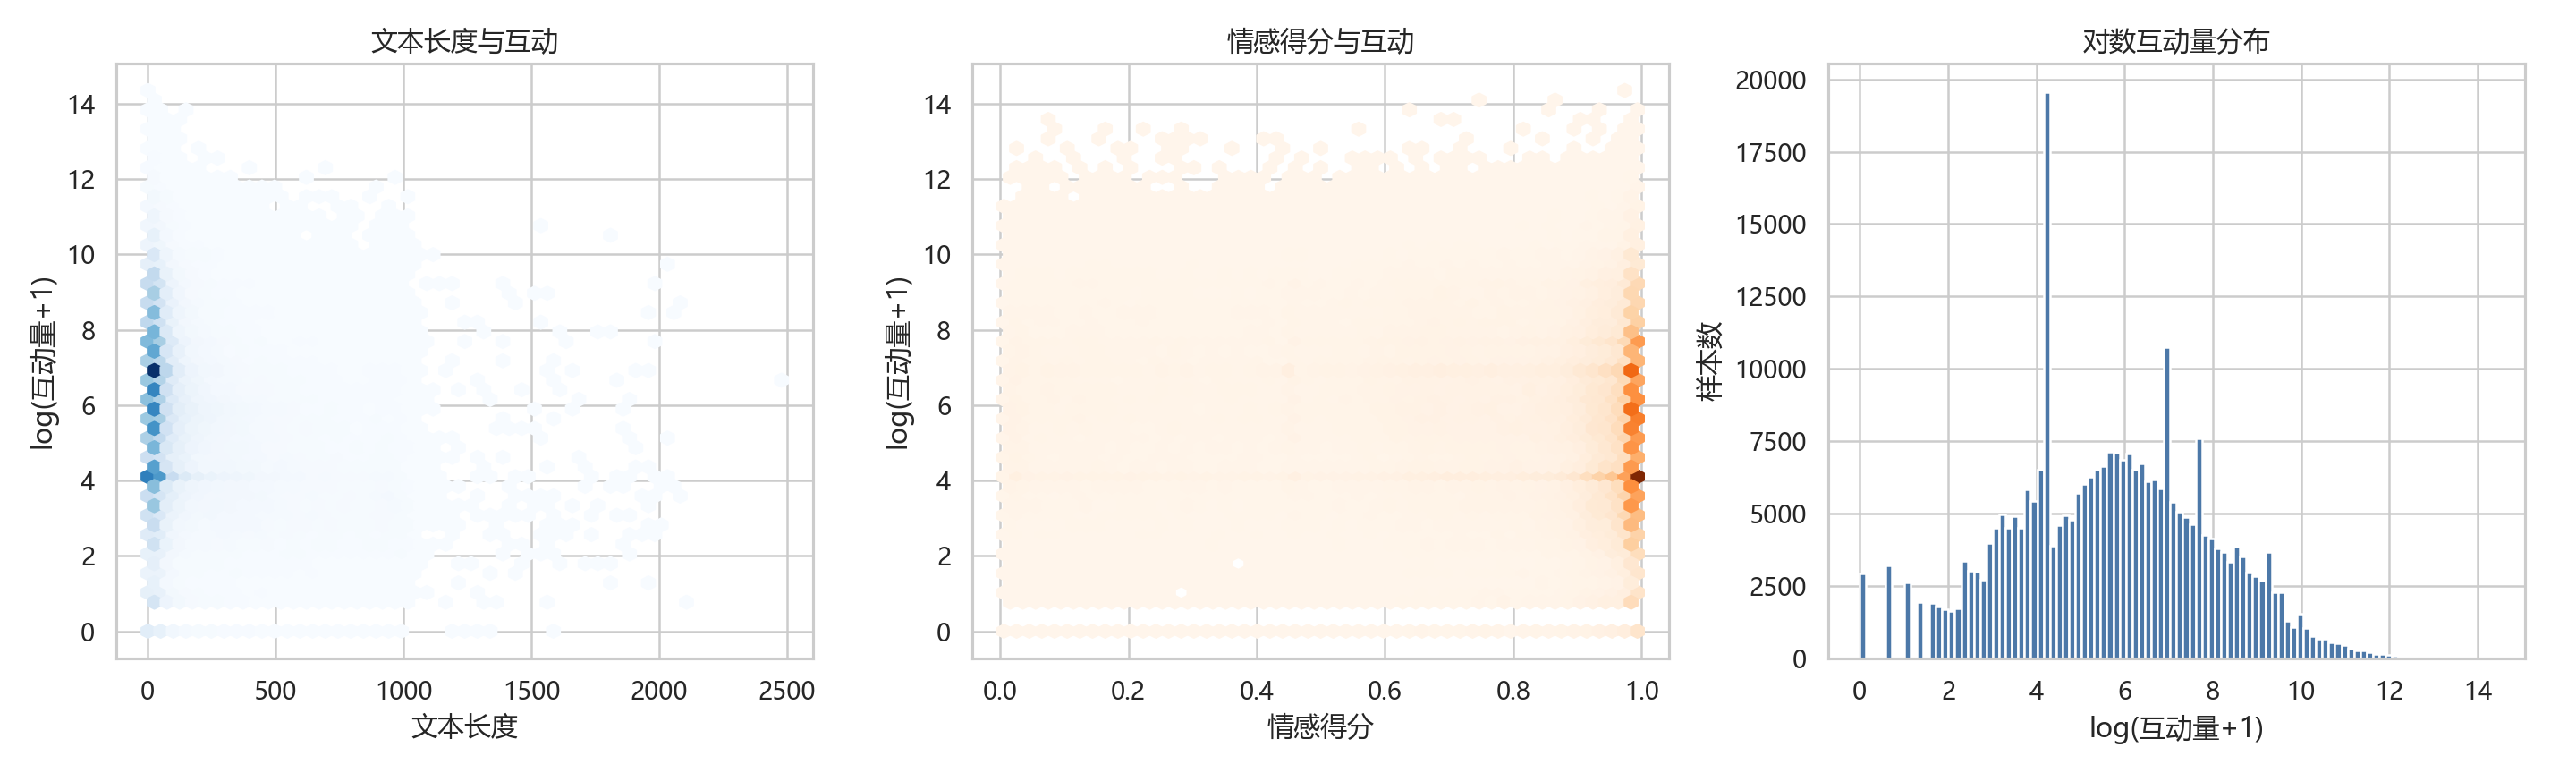
\includegraphics[width=\textwidth]{../outputs/chapter03/3_1_text_emotion_engagement.png}
    \caption{文本长度、情感得分与对数互动量的探索性分布}
    \label{fig:chapter3-text-overview}
\end{figure}

\subsection{文本情感与互动关系}
在情感维度上，本文进一步分析了情感强度与互动表现之间的关系。回归结果表明，情感变量与互动水平呈现负相关趋势。情感强度和情绪极端程度在主模型与稳健性模型中均表现为显著负相关，说明在本样本中，越偏离中性、越强烈的情绪表达，平均互动反而更低。
\subsection{互动分布特征}
从整体分布来看，笔记互动量呈现明显的长尾特征。大多数样本集中在较低互动区间，只有少量内容获得了极高互动。这也解释了为何本文对互动变量采用对数变换后再进行建模，以提高回归估计的稳定性并减弱极端值的影响。

\subsection{非线性趋势识别}
为了进一步识别长度变量与互动之间的非线性结构，本文对抽样样本进行了 LOWESS 平滑拟合。结果显示，文本长度与互动之间存在较明显的弯曲趋势，这说明简单线性模型不足以完整描述二者关系。因此，在后续 OLS 回归中，本文加入了长度平方项，以刻画可能存在的非线性效应。
\begin{figure}[H]
    \centering 
    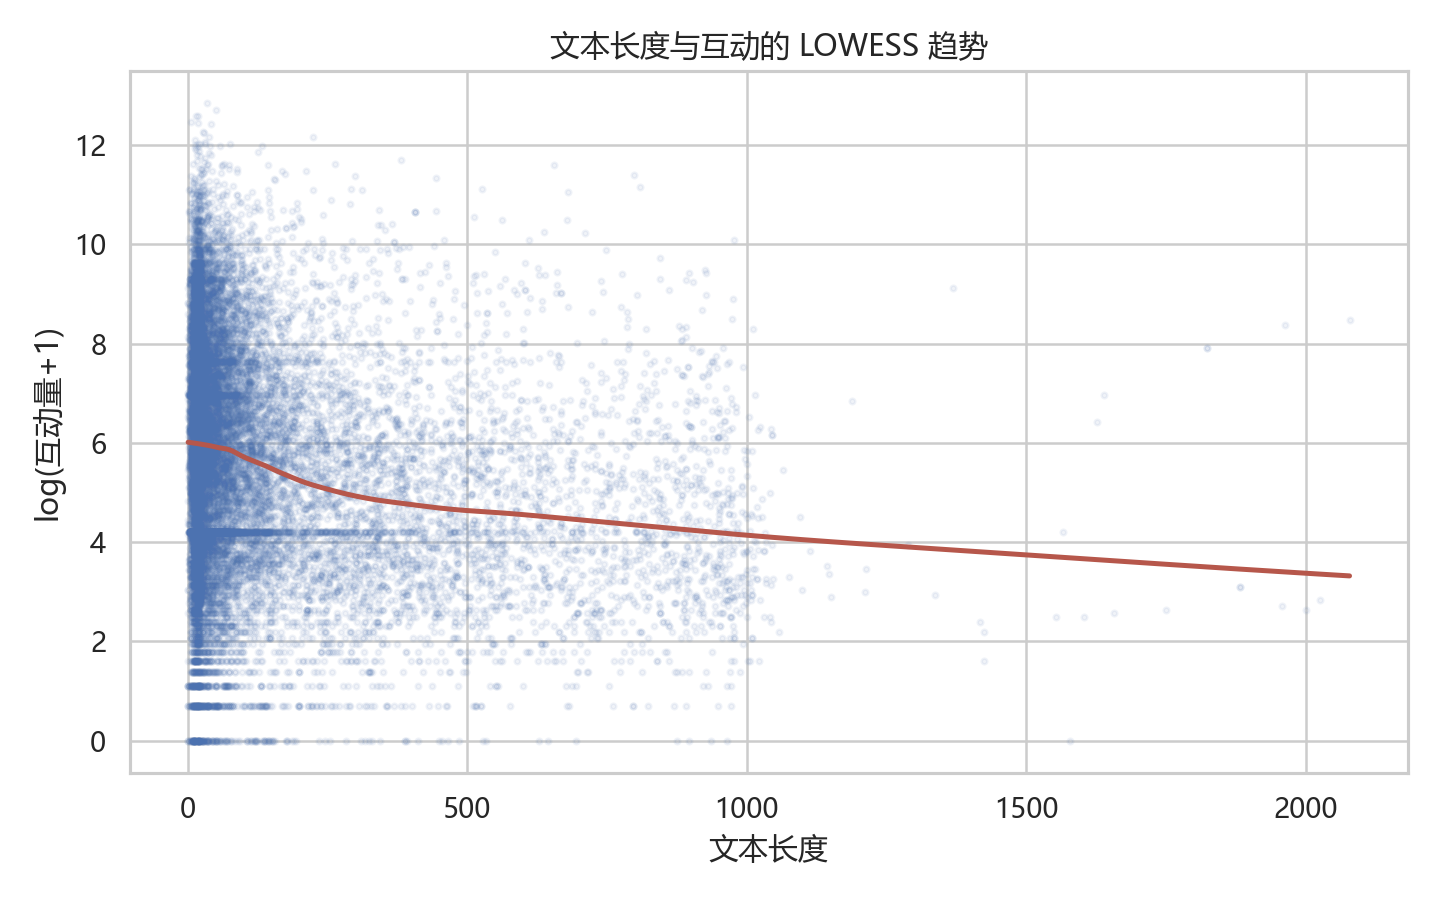
\includegraphics[width=0.8\textwidth]{../outputs/chapter03/3_1_content_length_lowess.png}
    \caption{文本长度与对数互动量的LOWESS趋势}
    \label{fig:length_lowess}
\end{figure}

\subsection{回归结果与稳健性检验}
在主回归模型中，本文以 
$engagement\_log$ 为因变量，以文本长度、长度平方项、情感强度、情绪极端程度和可读性为自变量进行 OLS 估计。结果显示，模型整体显著，但解释力有限，$R^2$约为0.050。这说明文本特征对互动具有统计意义上的解释力，但笔记热度仍受到账号属性、发布时间、封面质量、主题类别等其他因素影响。

具体而言，文本长度一次项系数显著为负，而二次项系数显著为正，说明长度关联具有非线性特征；情感强度与情绪极端程度的系数均显著为负，表明在本样本中，情绪越强或越极端，平均互动反而更低。可读性系数的绝对值很小，主模型中$p<0.001$，去除互动量最高1\%样本后为$p=0.018$；方向保持但证据减弱，不宜赋予较强的实际解释。

进一步地，本文剔除互动前1\%的极端值后重新估计模型，核心变量的方向和显著性基本保持一致，说明这些样本内关联并非完全由少数极端爆款观测驱动。不过，稳健性检验并未消除账号基础、主题与发布时间等潜在混杂因素，结果仍不应解释为因果效应。
\subsection{分组分析}
为更直观地观察长度关联，本文进一步将文本长度按分位数分组，比较不同长度区间的平均互动水平。结果表明，不同长度组的平均互动存在差异，整体形态与回归结果一致；但这些分组均值只能描述当前样本，不能直接据此确定普遍适用的“最优长度”。
\begin{figure}[H]
    \centering 
    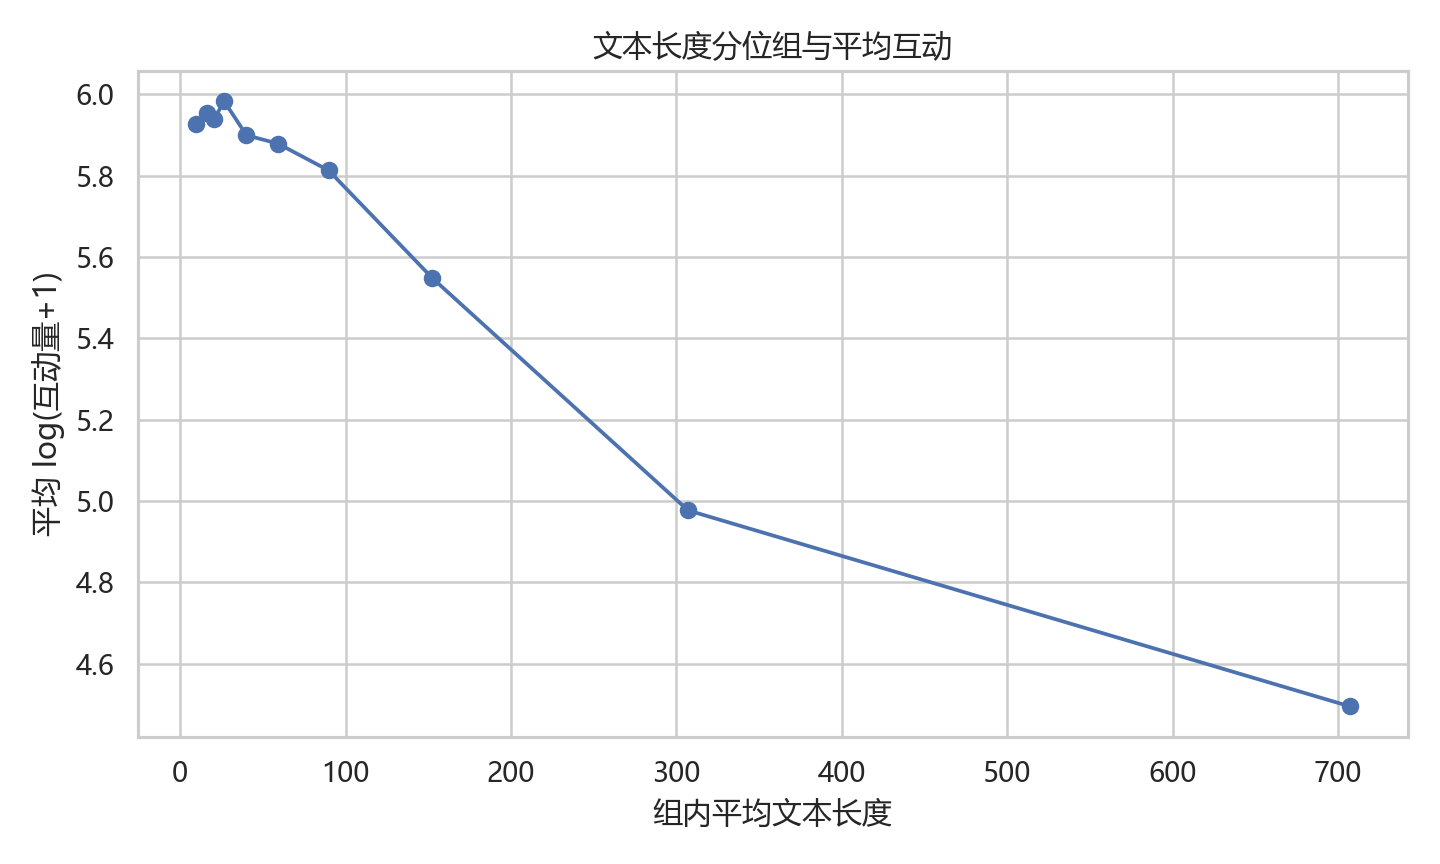
\includegraphics[width=0.8\textwidth]{../outputs/chapter03/3_1_length_groups.png}
    \caption{文本长度分位数组的互动表现}
    \label{fig:length_group_analysis}
\end{figure}

\subsection{情感分组结果}
最后，本文对情感强度与情绪极端程度进行了分组比较。结果表明，情感强度较低、情绪更接近中性的样本平均互动更高；而情绪极端程度越高，平均互动水平总体越低。这一结果与回归分析保持一致，进一步说明在小红书笔记场景中，过强或过于极端的情绪表达并不一定带来更高互动。

综合来看，文本长度与互动呈现非线性统计关系，情感强度及情绪极端程度总体上与互动负相关，可读性关联较弱且不够稳健。由于模型解释度较低且仍可能存在未观测混杂，本章将这些结果作为描述性与预测性证据，而不将其表述为内容特征对热度的确定性作用。

\section{主题相关性与信息价值分析}

在社交媒体中，内容传递的信息集中程度以及“标题---正文”间的词汇重合，可能与用户互动同时变化。本节基于 TF--IDF 算法提取文本核心词，从“信息密度”与“标题匹配度”两个维度考察其与互动表现的关联。

\subsection{变量构建与共线性修正}
为量化笔记的信息分布情况，本文首先利用 TF-IDF 算法提取单篇笔记中的高权重核心词汇。“信息密度（info\_density）”定义为正文高权重词汇数占局部总有效词数的比重；“标题匹配度（title\_match）”则定义为标题关键词与正文关键词的交集词数占标题总词数的比例，主要用于衡量笔记是直接“白描”还是存在一定的内容悬念差。

在将上述变量引入回归模型前，本文利用 Z-score 对连续型自变量进行标准化，再由标准化后的长度构造平方项。处理后，各变量的方差膨胀因子（VIF）介于1.12至7.88之间，模型总体条件数（Cond. No.）为8.64。个别变量仍存在中等程度的共线性，解释单个系数时需保持谨慎。

\subsection{信息价值回归结果与检验}
本文将标准化后的各特征变量纳入 OLS 回归模型，因变量为对数互动量，而非除以粉丝数后的互动率。回归估计结果如表 \ref{tab:ols_results_info} 所示。整体模型达到统计显著（F统计量 = 254.6，Prob(F) $< 0.001$），但$R^2$仅为0.071。

\begin{table}[H]
    \centering
    \caption{信息价值与互动表现的多元线性回归结果}
    \label{tab:ols_results_info}
    \begin{tabular}{lcccc}
        \toprule
        \textbf{变量} & \textbf{标准化系数 ($\beta$)} & \textbf{标准误(Std.Err)} & \textbf{t 值} & \textbf{P>|t|} \\
        \midrule
        截距项 (Intercept)     & 5.4294  & 0.021 & 254.91 & $<$0.001 *** \\
        内容长度 ($content\_len$)      & -0.5052 & 0.043 & -11.76 & $<$0.001 *** \\
        内容长度平方 ($content\_len^2$)& 0.0768  & 0.015 & 5.19   & $<$0.001 *** \\
        情感强度 ($emotion\_strength$) & -0.1138 & 0.018 & -6.23  & $<$0.001 *** \\
        极端情感 ($emotion\_extreme$)   & -0.0981 & 0.019 & -5.29  & $<$0.001 *** \\
        信息密度 ($info\_density$)      & 0.1057  & 0.025 & 4.23   & $<$0.001 *** \\
        标题匹配度 ($title\_match$)     & -0.1698 & 0.016 & -10.48 & $<$0.001 *** \\
        \midrule
        \multicolumn{5}{l}{样本量 = 20,000 \quad $R^2$ = 0.071 \quad 总体条件数(Cond. No.) = 8.64} \\
        \bottomrule
    \end{tabular}
    \vspace{1ex}
    \\
    \small{\textit{注：*** 代表 1\% 的显著性水平。}}
\end{table}

由于引入了标准化处理，相较于前述基础回归模型，本模型中的系数可用于比较不同特征与对数互动量的样本内关联强度。加入新特征后，长度的非线性形态及极端情绪的负向系数仍然存在；信息密度和标题匹配度则提供了两个额外的关联信号。这里的因变量是对数互动量而非互动率，系数也不代表因果作用。

\subsection{信息密度的“干货溢价”效应}
回归结果表明，信息密度与互动表现呈显著正相关（$\beta=0.1057, p<0.001$）。在控制模型中其他文本变量后，高权重词汇占比较高的笔记通常具有更高的平均互动量。这一结果与“信息更集中、更便于检索的内容可能更符合用户决策需求”的解释一致。不过，本文的信息密度来自TF--IDF阈值构造，且模型尚未控制全部账号与主题差异，因此该结果应理解为相关性证据，而非信息密度对互动的确定性因果效应。

\subsection{标题匹配度的负向关联及可能解释}
模型同时揭示了一个值得关注的反直觉现象：标题匹配度与互动表现呈显著负相关（$\beta=-0.1698, p<0.001$），且其标准化系数绝对值在模型中仅次于文本长度。这意味着，在当前样本和词汇重合度定义下，标题关键词被正文直接重复得越多，笔记的平均互动量反而越低。

这一现象可能与信息缺口或标题的悬念表达有关：过分直白的重复可能降低读者继续探索的意愿，而适度的信息差可能保留阅读动机。不过，当前指标衡量的是分词后的词汇重合，而不是严格的语义一致性；标题较短、正文缺失或不同主题的语言习惯也可能影响该指标。因此，“悬念留白”只能作为一种可能解释，尚不能由本模型直接验证。

\subsection{信息分布的可视化特征}
为直观呈现变量的联合分布，本文绘制信息密度、标题匹配度与互动强度的二维六边形密度图（Hexbin Plot）。如图 \ref{fig:info_hexbin} 所示，信息密度较高的部分区间延伸至较高互动区域，而标题匹配度较高区域的样本更多集中在较低互动水平。该图与回归系数方向一致，但二维分布仍会受到粉丝规模、主题和文本长度等变量影响，不能单独验证“干货溢价”或“悬念留白”等行为机制。

\begin{figure}[H]
    \centering 
    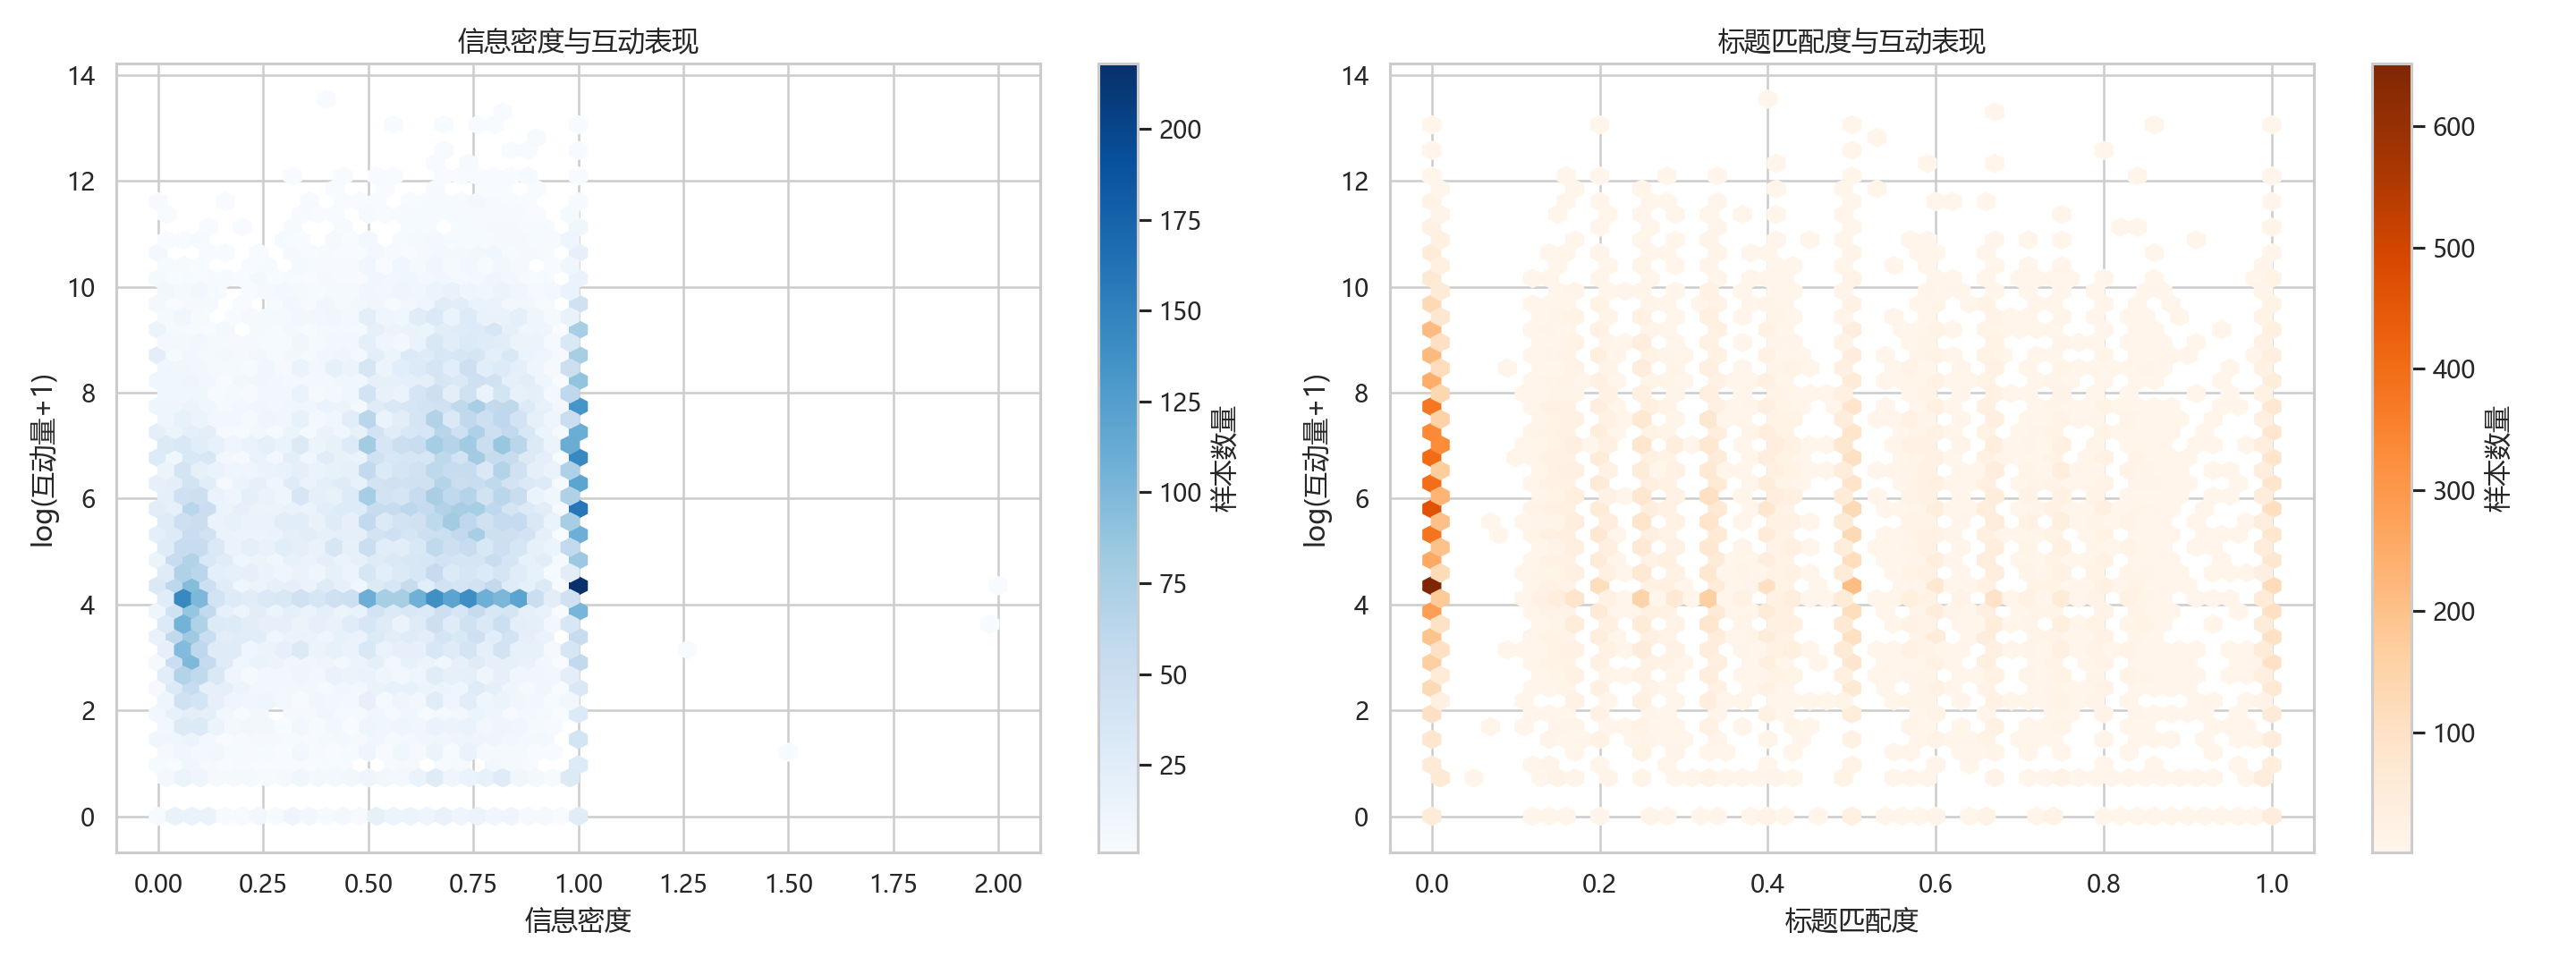
\includegraphics[width=0.8\textwidth]{../outputs/chapter03/3_2_info_value_hexbin.png}
    \caption{信息密度、标题匹配度与互动量的二维密度分布}
    \label{fig:info_hexbin}
\end{figure}

\chapter{笔记形式特征与多媒体数据边界}

\section{多媒体数据的可用性审计}
小红书具有明显的视觉内容属性，但视觉重要性并不意味着当前数据可以支持视觉效果评估。仓库内的结构化明细表以标题、正文、标签、互动量、粉丝量、时间和地点等字段为主；部分批次虽保留媒体链接或类型文本，却没有与每条笔记稳定对应的原始图片、视频文件、视频时长、字幕或背景音乐等元数据。链接还可能随时间失效，无法作为可重复实验的固定输入。

因此，本轮研究没有计算图片数量、色彩、构图、清晰度、美学质量、视频时长或完播率，也不报告“图片越多”“视频存在最优时长”等未经验证的结论。分类与回归实验中的10项输入特征均来自发布前可获得的结构化字段，不包含视觉特征。若后续补充媒体资产，应先用笔记唯一标识校验图文配对，并记录抓取时间与缺失机制；在同一数据切分上提取色彩、清晰度、视觉语义和视频元数据后，才能与当前结构化基准进行增量比较。

\section{当前可复现的文本形式特征}
现有数据能够稳定构造的形式变量包括标题长度、正文长度、标签数量、感叹号数量、问号数量、Emoji数量以及标题---正文词汇重合度。这些指标描述的是文本表层结构，不等同于完整排版质量：CSV中的换行、富文本加粗和平台端渲染样式未必被一致保留，因此本研究没有推断分段质量、视觉层级或阅读停留时间。

第8章的统一相关性分析显示，标签、Emoji、感叹号和问号等变量与互动量的Spearman相关系数绝对值均小于0.05；部分检验在大样本下达到统计显著，但实际效应较弱。它们仍作为低成本结构化特征进入后续模型，用于检验与粉丝量、文本长度、情感及时间变量组合后是否提供预测增量。无论相关性还是模型重要性，都不能证明增加某种符号或改变格式必然提高互动。

\chapterimage{chapter_head_2.pdf}
\chapter{发布者基础影响力与用户数据边界}

\section{粉丝规模与互动的描述性关联}
当前归档能够较稳定使用的发布者变量是采集时展示的粉丝数量。鉴于该变量呈明显长尾分布，相关性与模型分析均使用$\log(1+\text{fans})$。图\ref{fig:followers_likes}按粉丝数分位组展示平均点赞数：从Q1到Q5，组均值总体递增。这是一个清晰的描述性梯度，但不能据此断言粉丝增长会按相同比例带来点赞增长，因为账号主题、内容质量、发布时间与平台推荐均可能同时影响二者。

\begin{figure}[htbp]
    \centering
    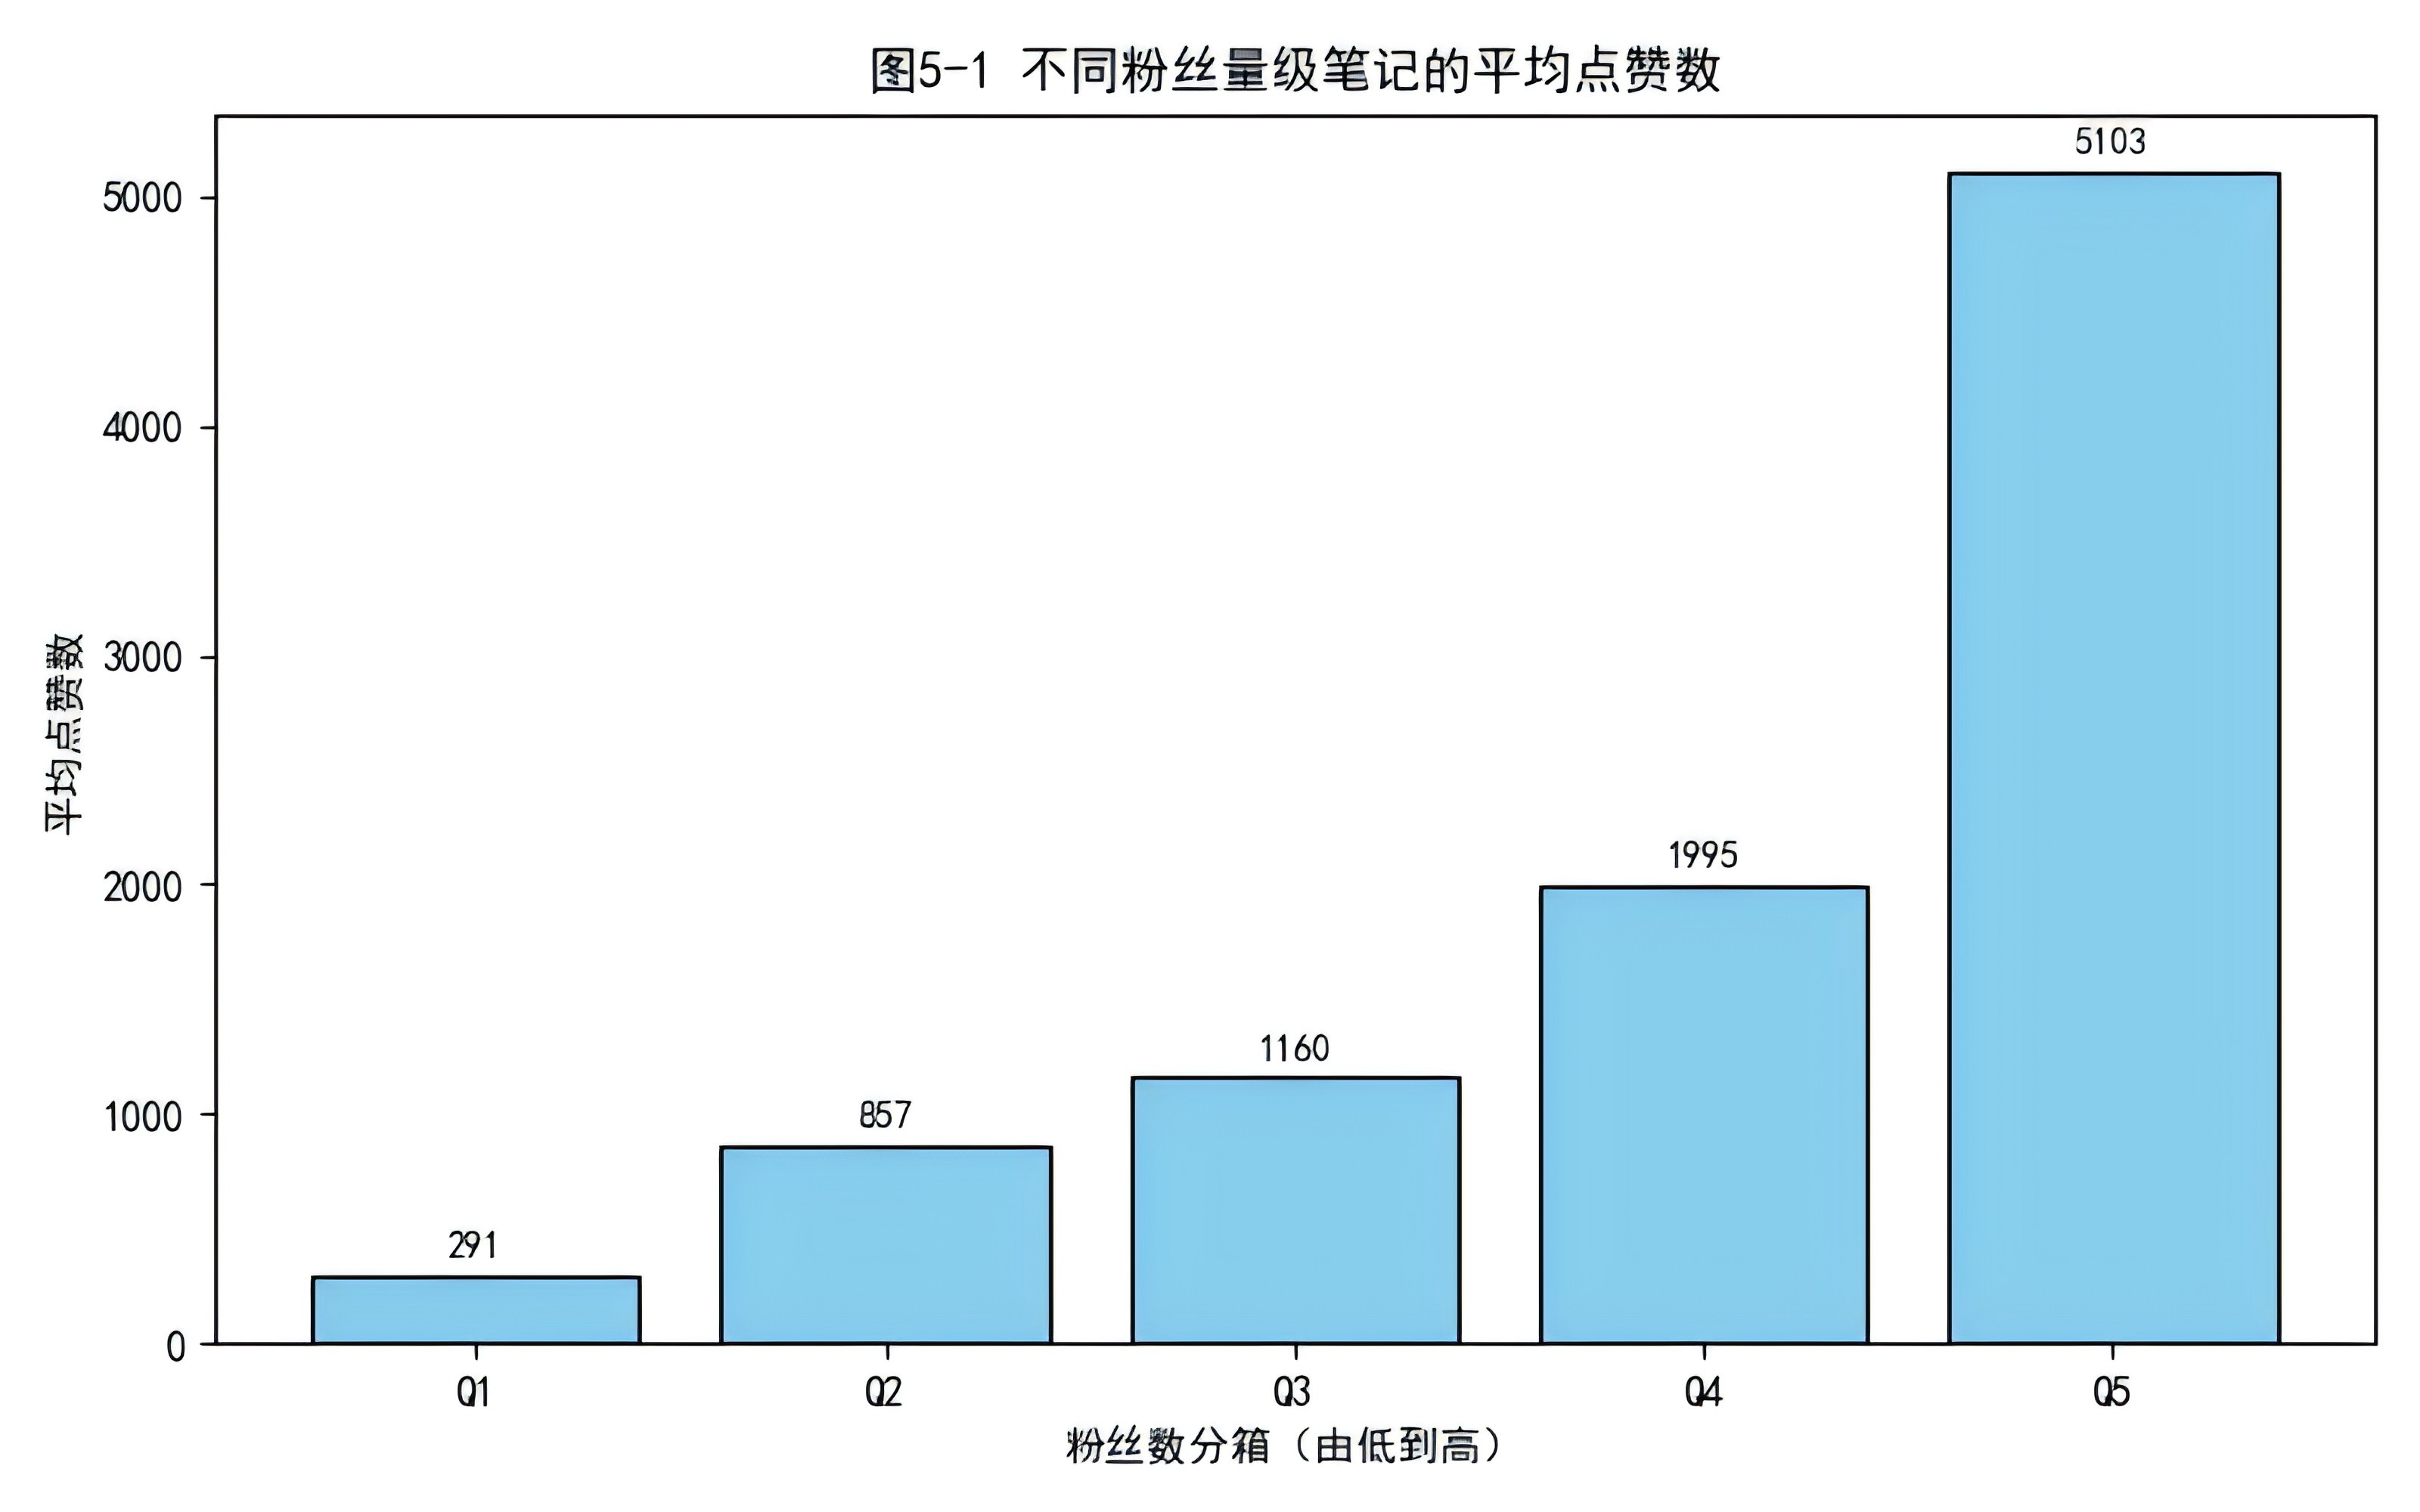
\includegraphics[width=0.8\textwidth]{16.png}
    \caption{不同粉丝量级笔记的平均点赞数（描述性分组）}
    \label{fig:followers_likes}
\end{figure}

在统一去重后的相关性样本中，粉丝数对数与对数互动量的Pearson和Spearman相关系数分别为0.489和0.469；爆款组与普通组的粉丝数对数差异对应Cohen's $d=0.696$。这些结果表明粉丝规模是当前字段中最稳定的关联信号之一。后续随机森林分类和梯度提升回归也将其识别为主要预测特征，但预测重要性仍不等于因果效应。

\section{未纳入的用户历史、认证与社交网络变量}
当前数据不能稳定构造发布者在每条笔记发布前7天、30天或90天的完整历史表现，也没有一致的认证状态、粉丝人口属性和用户---笔记交互边。因此，本轮研究没有填补或模拟以下变量：历史平均点赞与发帖频率、企业号或达人认证、账号内容垂直度、粉丝画像及社交网络中心性。若以采集后的互动反推发布前历史，还会造成时间泄漏。

未来若补充按时间排序且覆盖完整的发布者历史，可只使用每条样本发布时间之前的记录构造滚动统计，并用作者分组或时间外切分验证；内容垂直度可基于历史主题分布的熵值定义，认证与粉丝画像则必须来自明确、合法且可审计的字段。在这些数据到位前，本章不对“高垂直度更忠诚”或“认证带来额外流量”等命题给出实证结论。

\chapterimage{chapter_head_2.pdf}
\chapter{发布时机与上下文分析}

本章对具有可解析发布日期或发布地点的记录进行探索性分组，比较星期、日期类型与省份之间的互动差异。章节中的样本筛选服务于对应图表，与后文统一去重的建模样本口径不同；“高粉丝、低互动”规则仅用于异常值敏感性检查，不被解释为真实的买粉标签。以下结果反映的是同期样本的条件关联，而非发布时机或地域对互动的因果效应。

\section{星期分组的互动差异}
单因素方差分析显示，不同星期组的对数互动量存在统计差异（$F=946.56$，$p<0.001$，$\eta^2=0.018$）。效应量$\eta^2$表明星期仅解释约1.8\%的组间变异：样本量较大使检验容易达到显著，但星期本身的实际解释力有限。

在该探索性样本及平均对数互动指标下，周一均值最高（5.95），周五最低（5.01）；Tukey HSD事后比较也显示周五与多个日期组存在显著差异。该结果只能说明不同星期发布的样本构成和互动水平不同。内容类别、账号规模、采集批次与推荐流量都可能造成组间差异，现有数据不足以验证“心理补偿”“线上线下替代”等具体行为机制。第8章使用严格去重样本和爆款比例得到的星期排序略有不同，也说明结论会随指标和样本口径变化。

\begin{figure}[H]
    \centering
    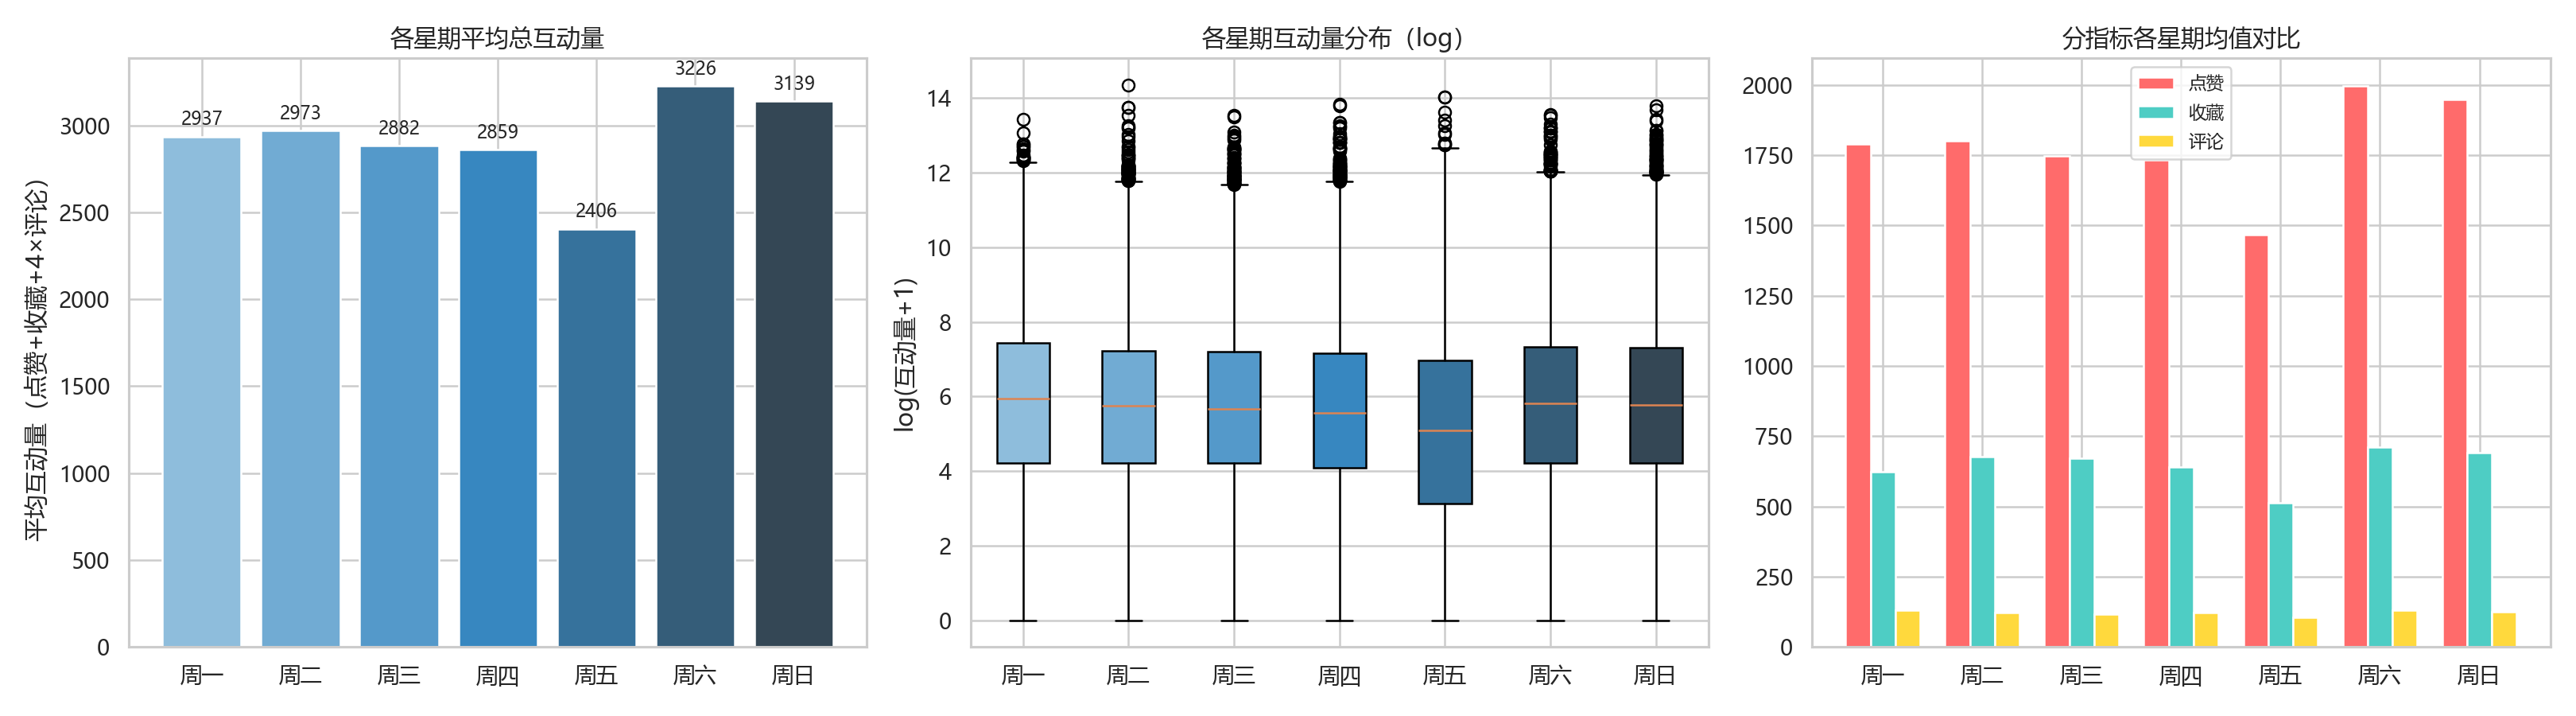
\includegraphics[width=\textwidth]{../outputs/chapter06/6_1_weekday_effect.png}
    \caption{不同星期组的笔记互动分布}
    \label{fig:weekday_effect}
\end{figure}

\section{节假日与调休日期的分组差异}
本文依据公开日历将可解析日期划分为普通工作日、普通周末、法定节假日和调休工作日。四组的ANOVA检验显示均值存在差异（$F=305.53$，$p<10^{-190}$）。在该样本中，调休工作日的平均总互动为4,744、平均对数互动为6.28，法定节假日的平均总互动为4,202；节假日与非节假日的Welch检验亦达到统计显著（$t=18.75$，$p<0.001$）。

上述均值是描述性结果。原始互动量长尾明显，少量爆款可能显著抬高组均值；同时，日期类型与主题、营销活动、账号结构和采集批次可能共同变化。由于数据不含曝光量、浏览频率和连续早期互动轨迹，本研究不能据此推断调休导致用户浏览增加，也不能将某类日期视为确定性的发布优势。

\begin{figure}[H]
    \centering
    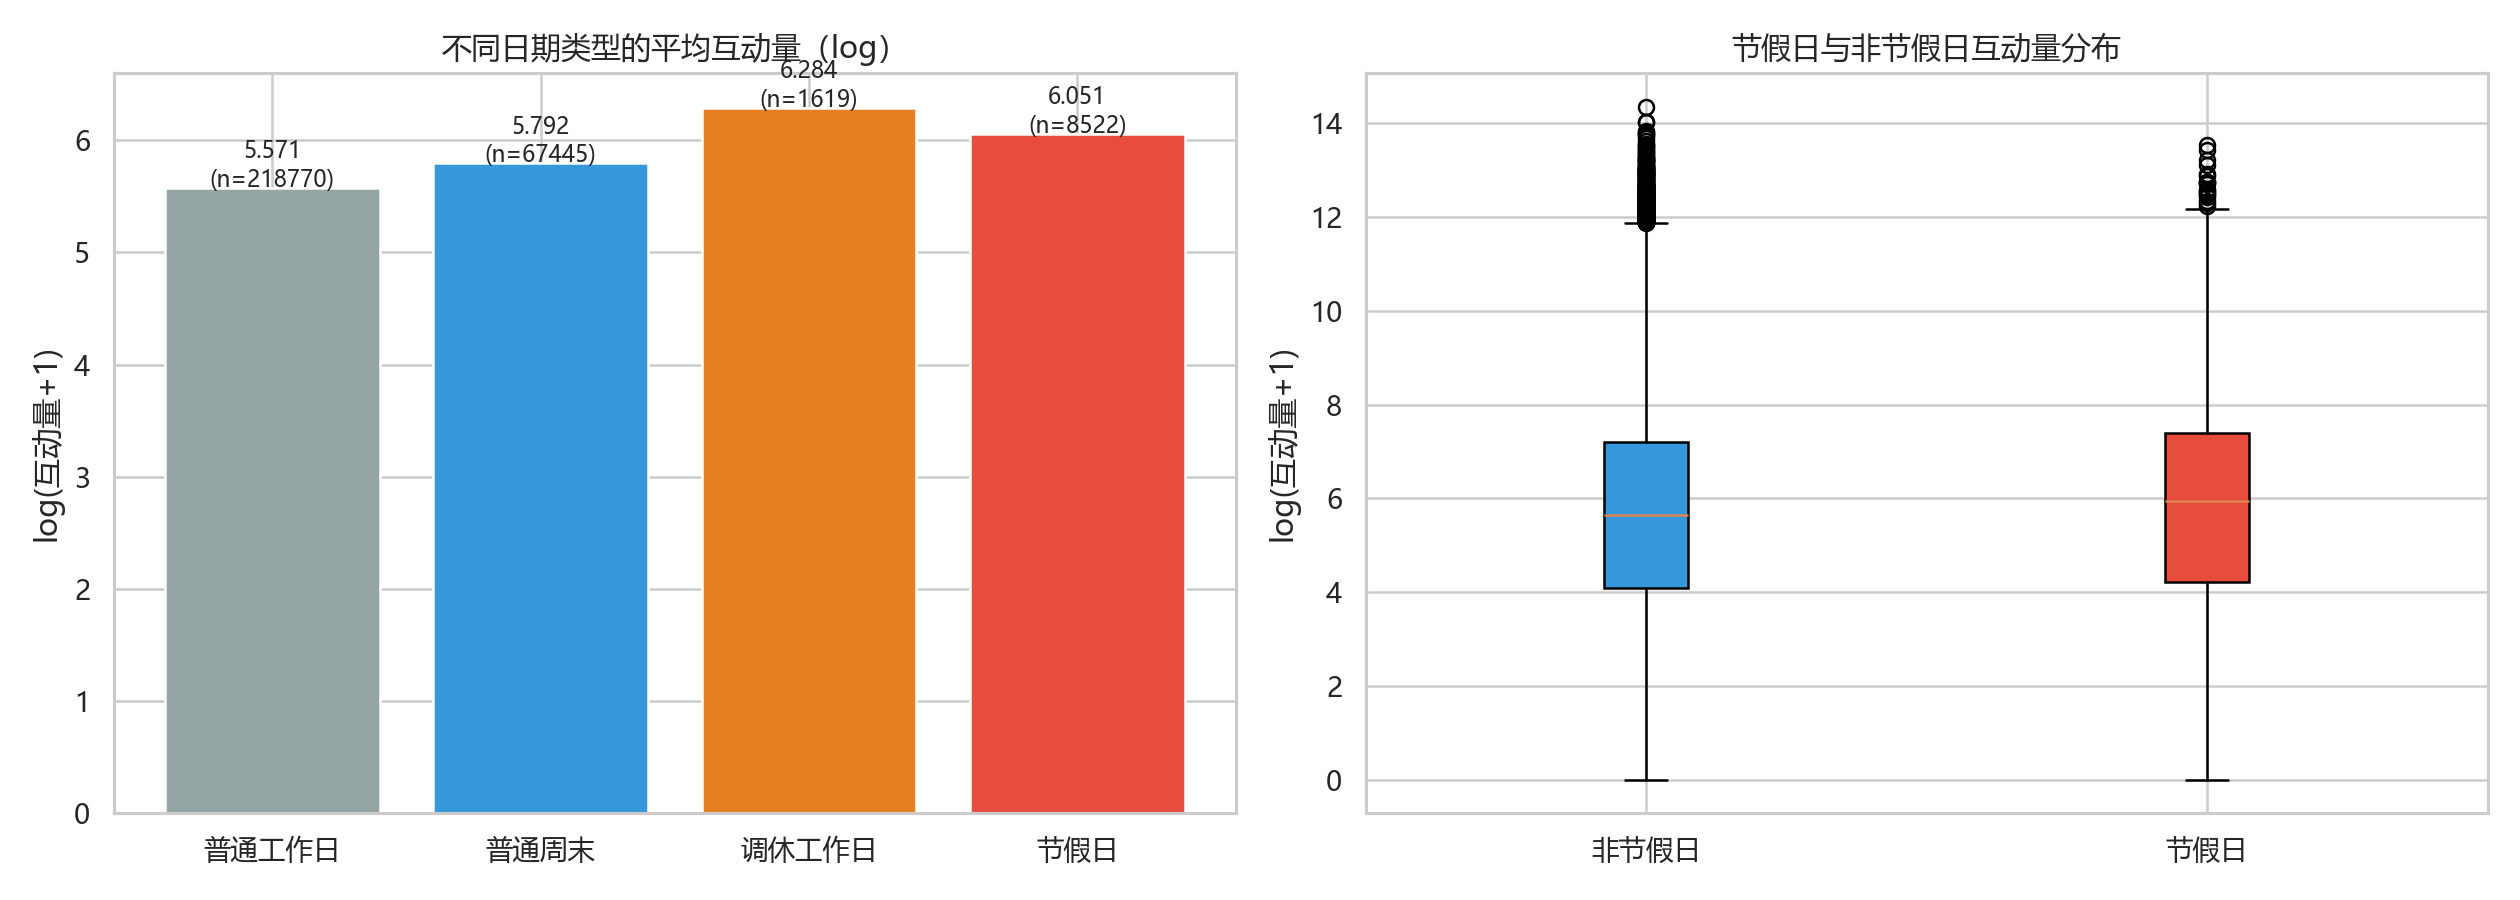
\includegraphics[width=0.8\textwidth]{../outputs/chapter06/6_1_holiday_effect.png}
    \caption{不同日期类型的互动表现分布}
    \label{fig:holiday_effect}
\end{figure}

\section{发布地点的样本分布与互动差异}
发布地点为用户自行展示且存在大量缺失，其含义可能是发布地、常驻地或内容标注地。本文在剔除空值和无法识别的文本后，对样本量较多的省级地区进行描述。广东样本最多，为25,624条；其平均对数互动为5.23。浙江、四川和上海的平均对数互动分别为5.97、5.88和5.87，在图示地区中相对较高。

这些差异不能直接归因于地区经济、代运营产业或生活方式文化。不同地区的领域构成、账号粉丝规模及地点填写倾向均可能不同，且地点缺失并非随机。因而图\ref{fig:province_analysis}用于呈现样本覆盖和组均值，不作为地域文化或产业链影响的因果证据。

\begin{figure}[H]
    \centering
    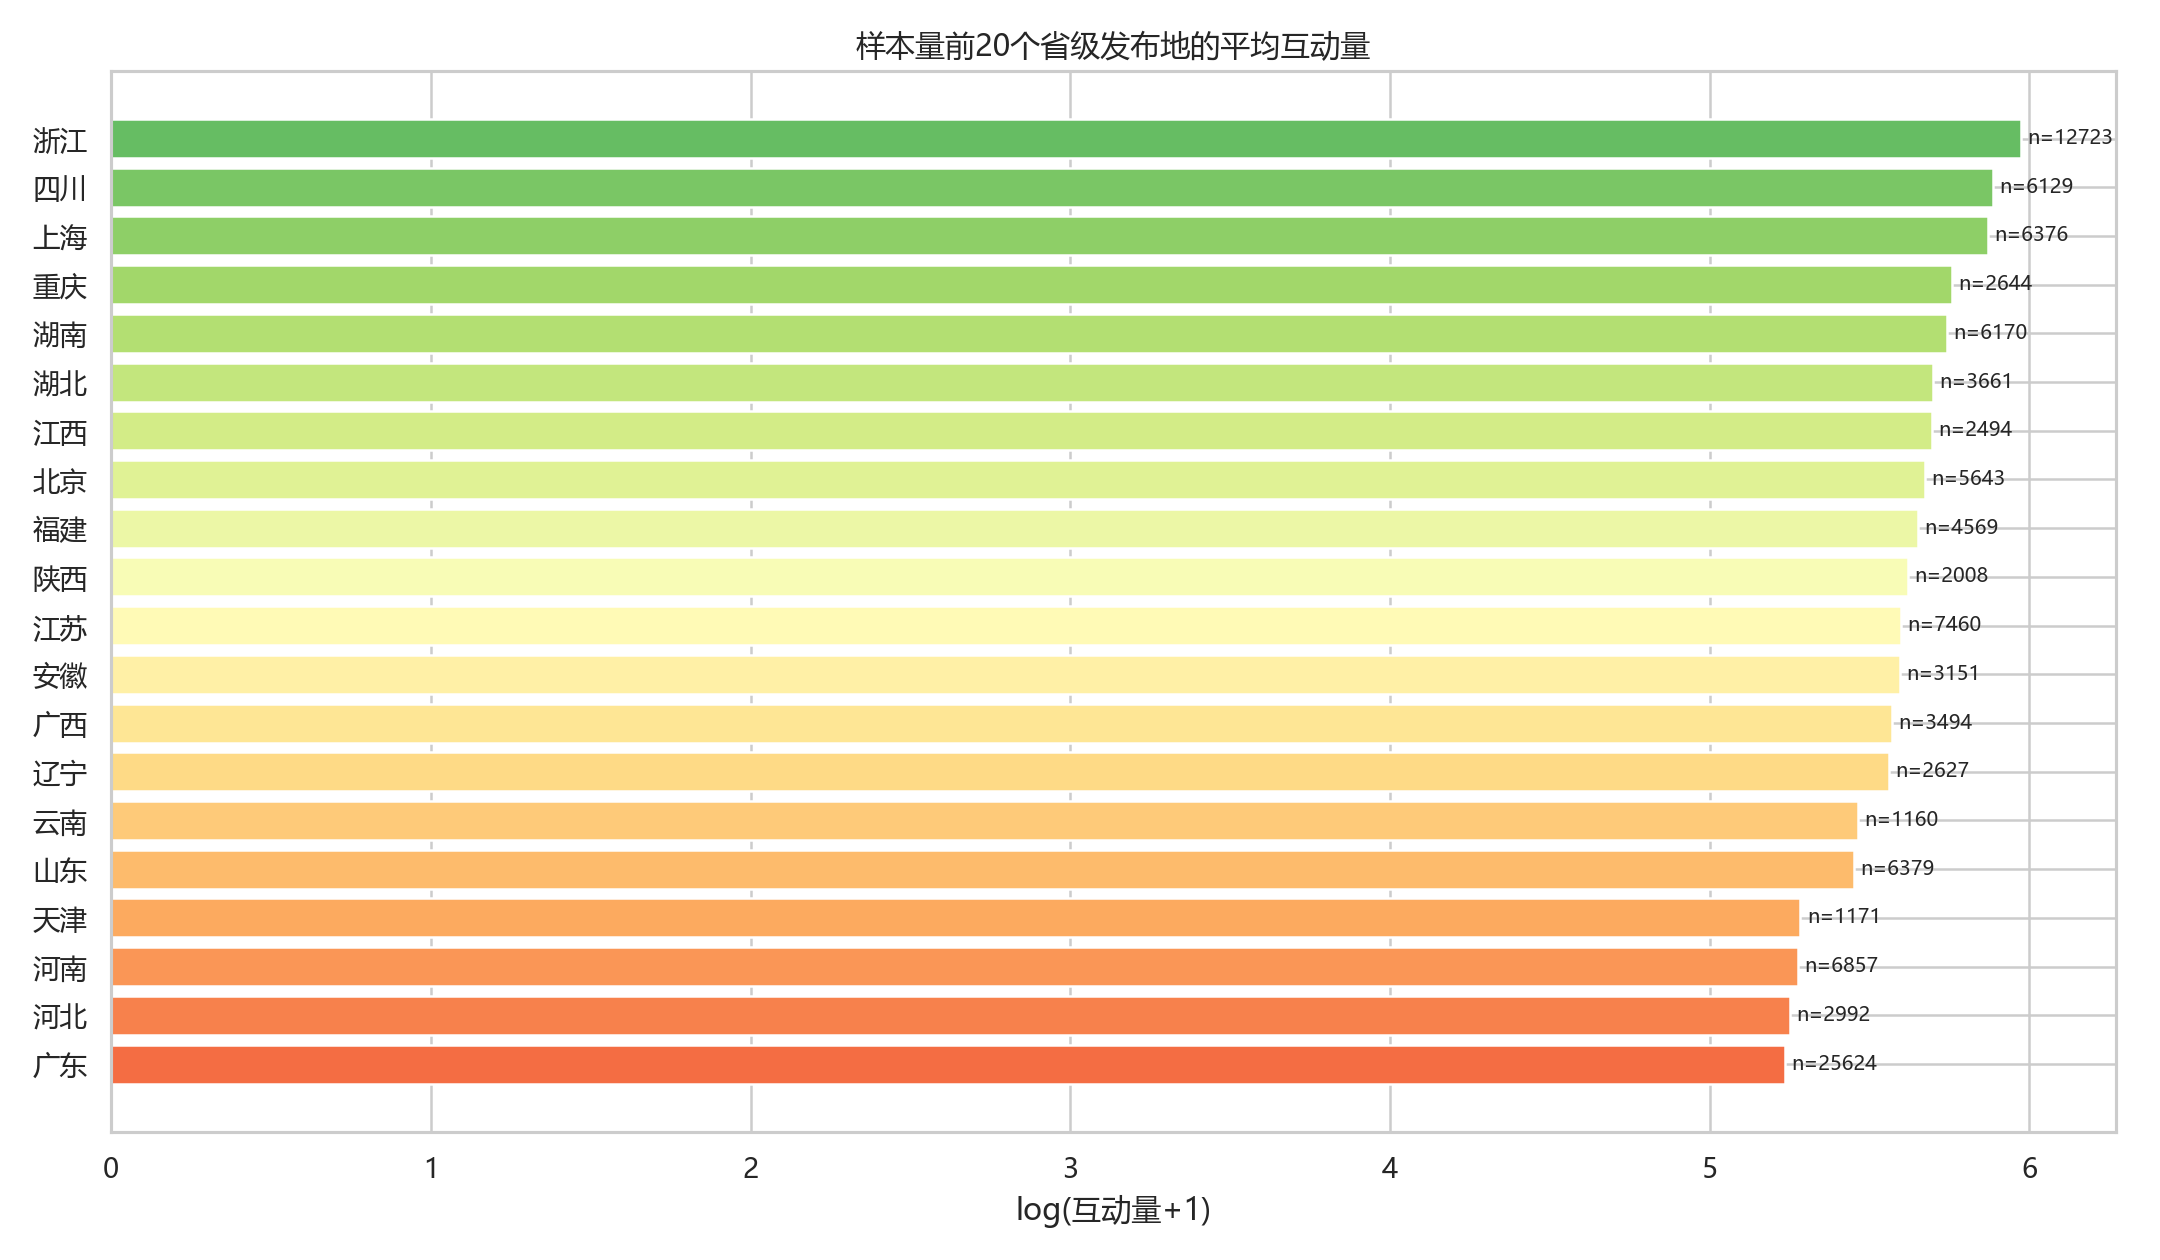
\includegraphics[width=\textwidth]{../outputs/chapter06/6_1_province_analysis.png}
    \caption{发布地点样本量与互动水平的描述性比较}
    \label{fig:province_analysis}
\end{figure}

\chapterimage{chapter_head_2.pdf}
\chapter{标签数量分析与话题数据边界}

\section{标签数量的描述性结果}
现有明细表能够从标签字段计算每篇笔记的标签数量。图\ref{fig:tag_count_likes}按标签数分组后显示，0--2个、3--4个、5--6个、7--10个和超过10个标签的笔记，平均点赞数依次约为2,358、2,119、2,047、1,422和1,586。该样本中的组均值并未呈现“标签越多点赞越高”的关系。

\begin{figure}[htbp]
    \centering
    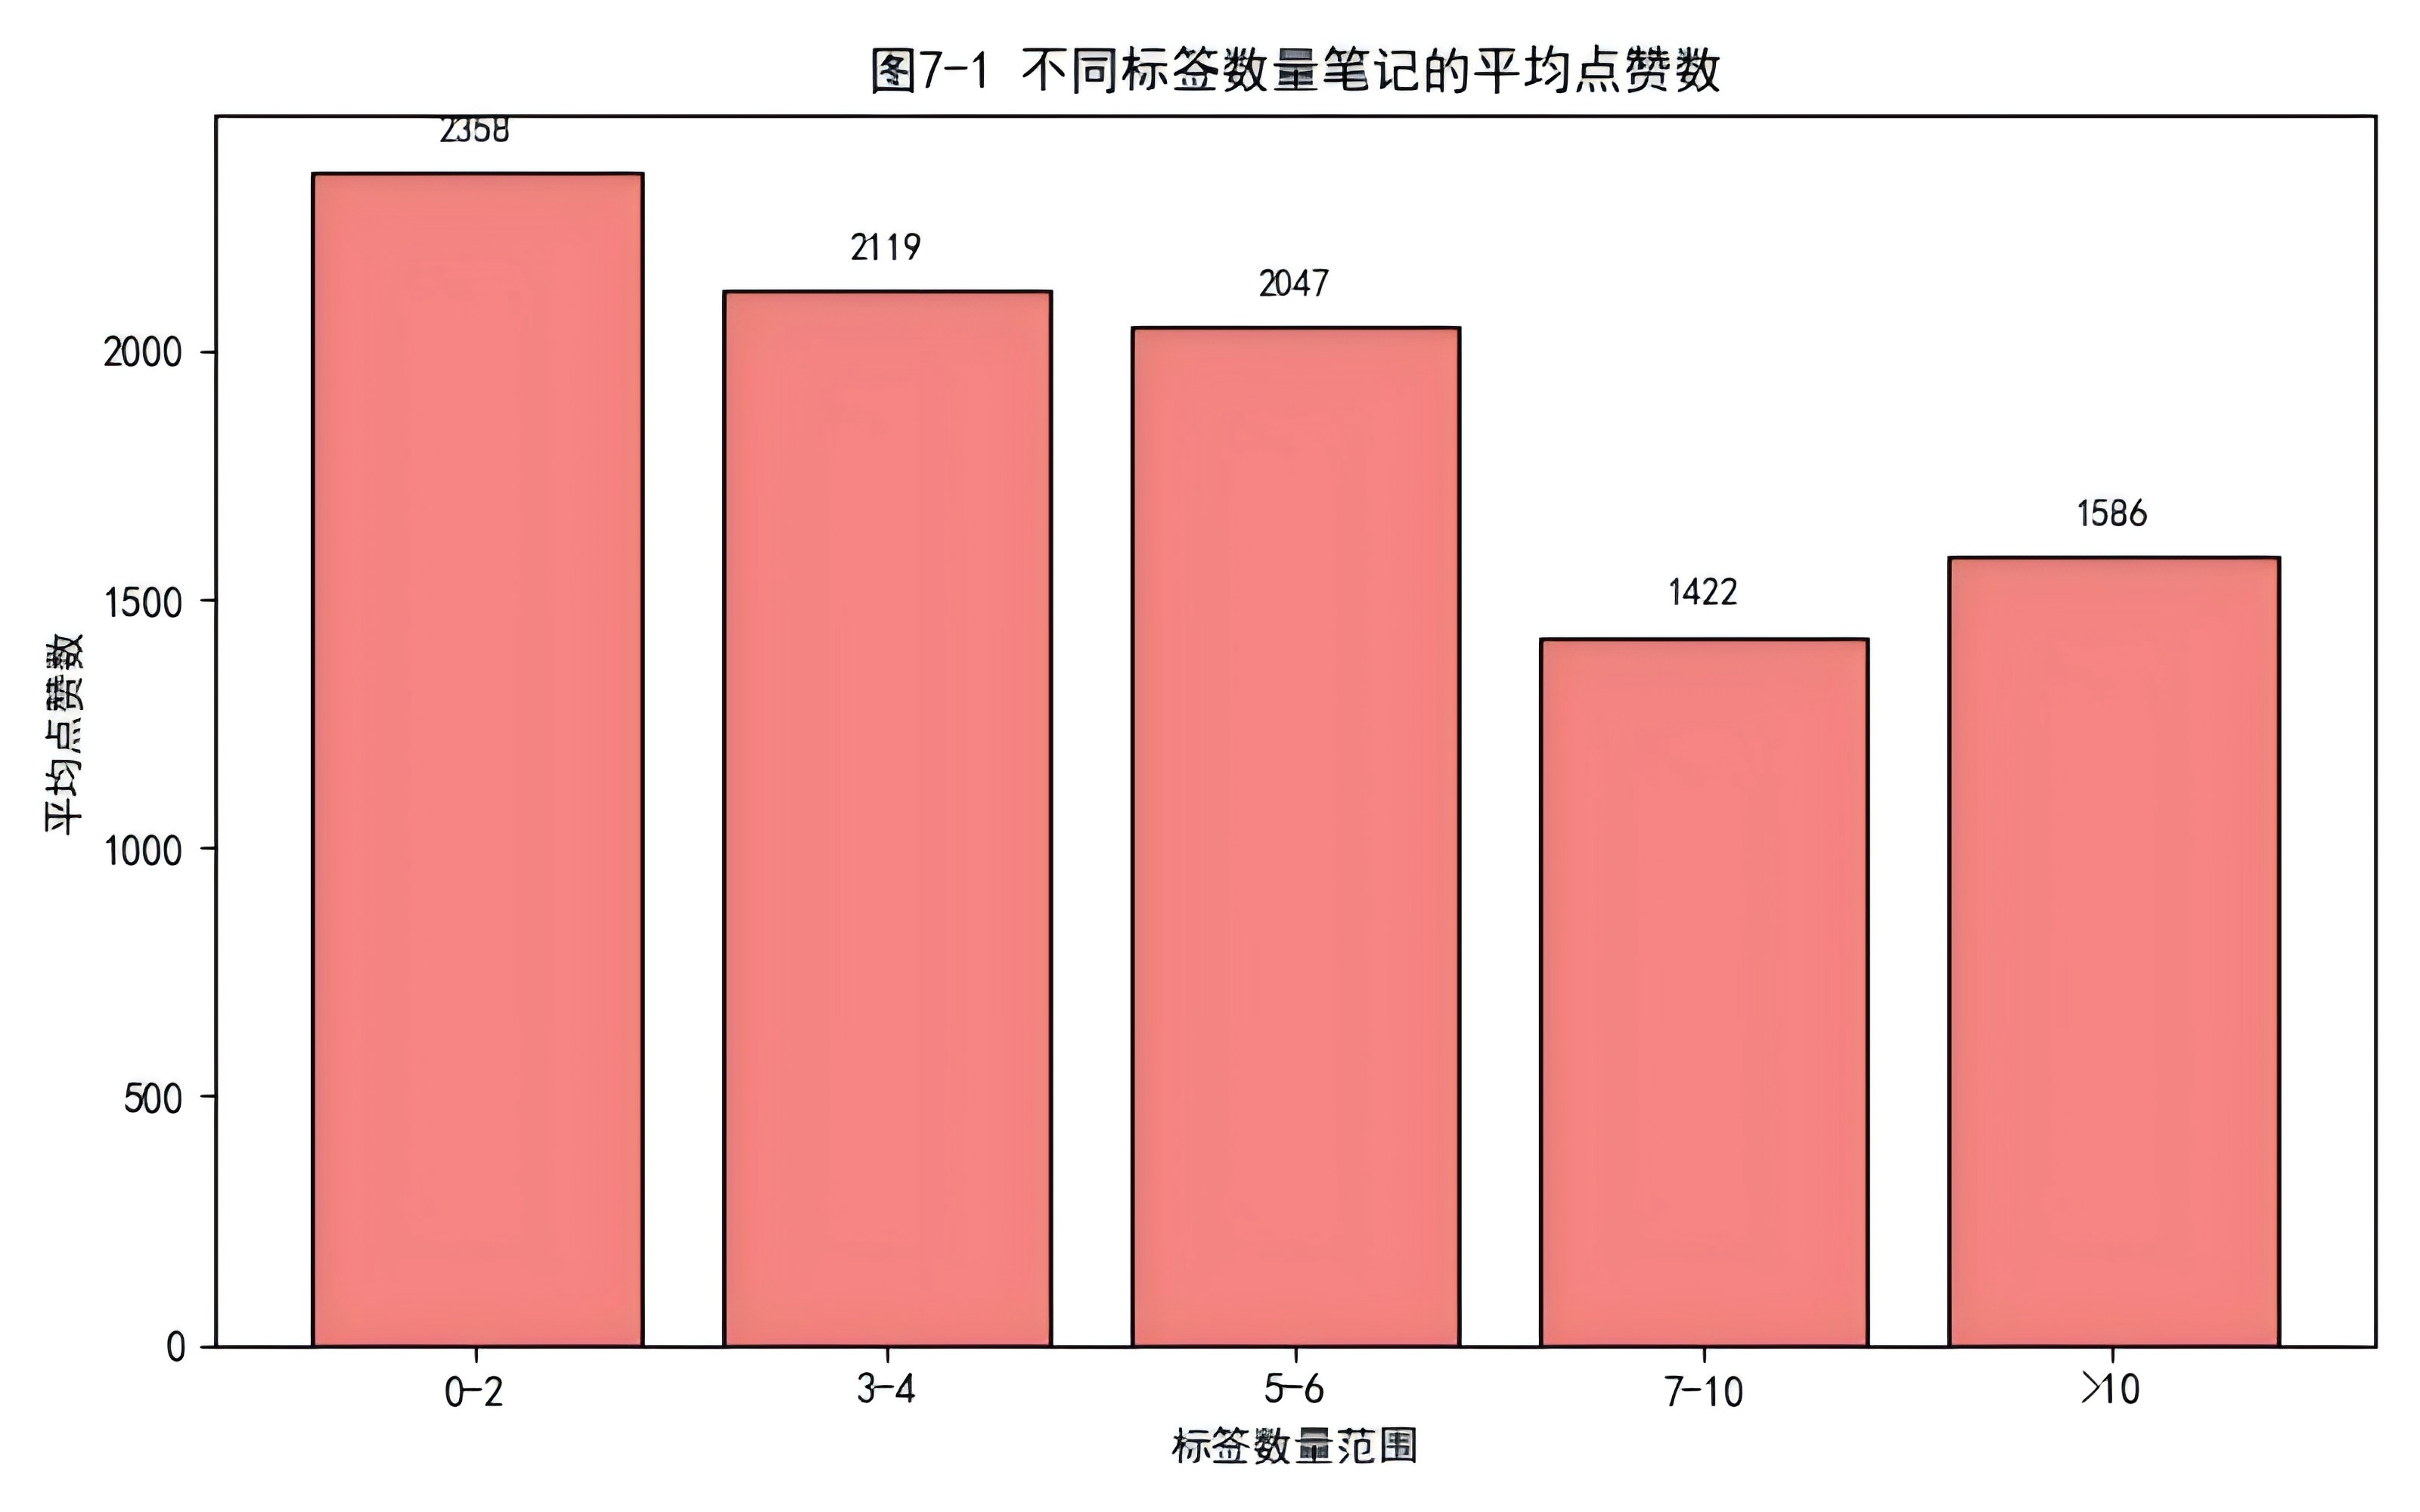
\includegraphics[width=0.8\textwidth]{17.png}
    \caption{不同标签数量笔记的平均点赞数（描述性分组）}
    \label{fig:tag_count_likes}
\end{figure}

统一相关性分析进一步表明，标签数量与互动量的相关系数绝对值较小，爆款组与普通组的标准化差异也较弱。标签数量可能同时反映领域习惯、账号策略和文本长度，简单组均值没有控制这些混杂因素。因此，本研究不把0--2个标签解释为普遍最优方案，也不依据该图给出确定性的标签数量建议。

\section{标签类型与热点响应的识别边界}
当前归档没有经过人工验证的标签类型词典、外部热点事件时间线，也没有笔记发布后0--72小时的连续互动快照。基于单次采集的最终互动量，无法可靠识别笔记何时介入热点，更无法估计热点响应的净效应或衰减曲线。因此，本轮没有实施“黄金标签组合”挖掘、倾向得分匹配、逆概率加权或热点生命周期建模，也不报告相关数值结果。

后续若补充可追溯的热点事件表和连续互动快照，可预先定义热门、垂直、地点及品牌标签，记录事件起止时间，再在严格时间切分下比较介入阶段。即使使用匹配或加权方法，也需检验共同支持与未观测混杂，不能仅凭方法名称将观察性差异表述为因果效应。

\chapterimage{chapter_head_2.pdf}
\chapter{多维度相关性分析}

\section{特征间相关性分析}
为避免原始文件、筛选文件及中间结果重复计入，本章仅读取文件名中包含“笔记详细信息”的数据，并优先按照笔记链接去重；链接缺失时，采用编号、标题和博主名称的组合去重。完成互动指标清洗后，共得到182,103条可用笔记，其中168,323条具有有效粉丝数。由于现有数据不包含可靠的图片数量、认证状态和发布小时，本章不对这些变量进行推断，而使用实际可获得的粉丝数、文本长度、标签数、标点与表情符号、情感得分、标题正文重合度、星期和地点完整性等特征。

考虑到互动量和粉丝数均呈明显长尾分布，本文分别构造
\[
 y=\log(1+\text{engagement}),\qquad
 x_{fans}=\log(1+\text{fans}),
\]
并同时计算Pearson相关系数与Spearman秩相关系数。前者用于识别线性关系，后者对极端值更稳健，可用于判断变量之间是否存在稳定的单调关系。图\ref{fig:chapter8_pearson}给出了特征间Pearson相关系数矩阵。

\begin{figure}[H]
    \centering
    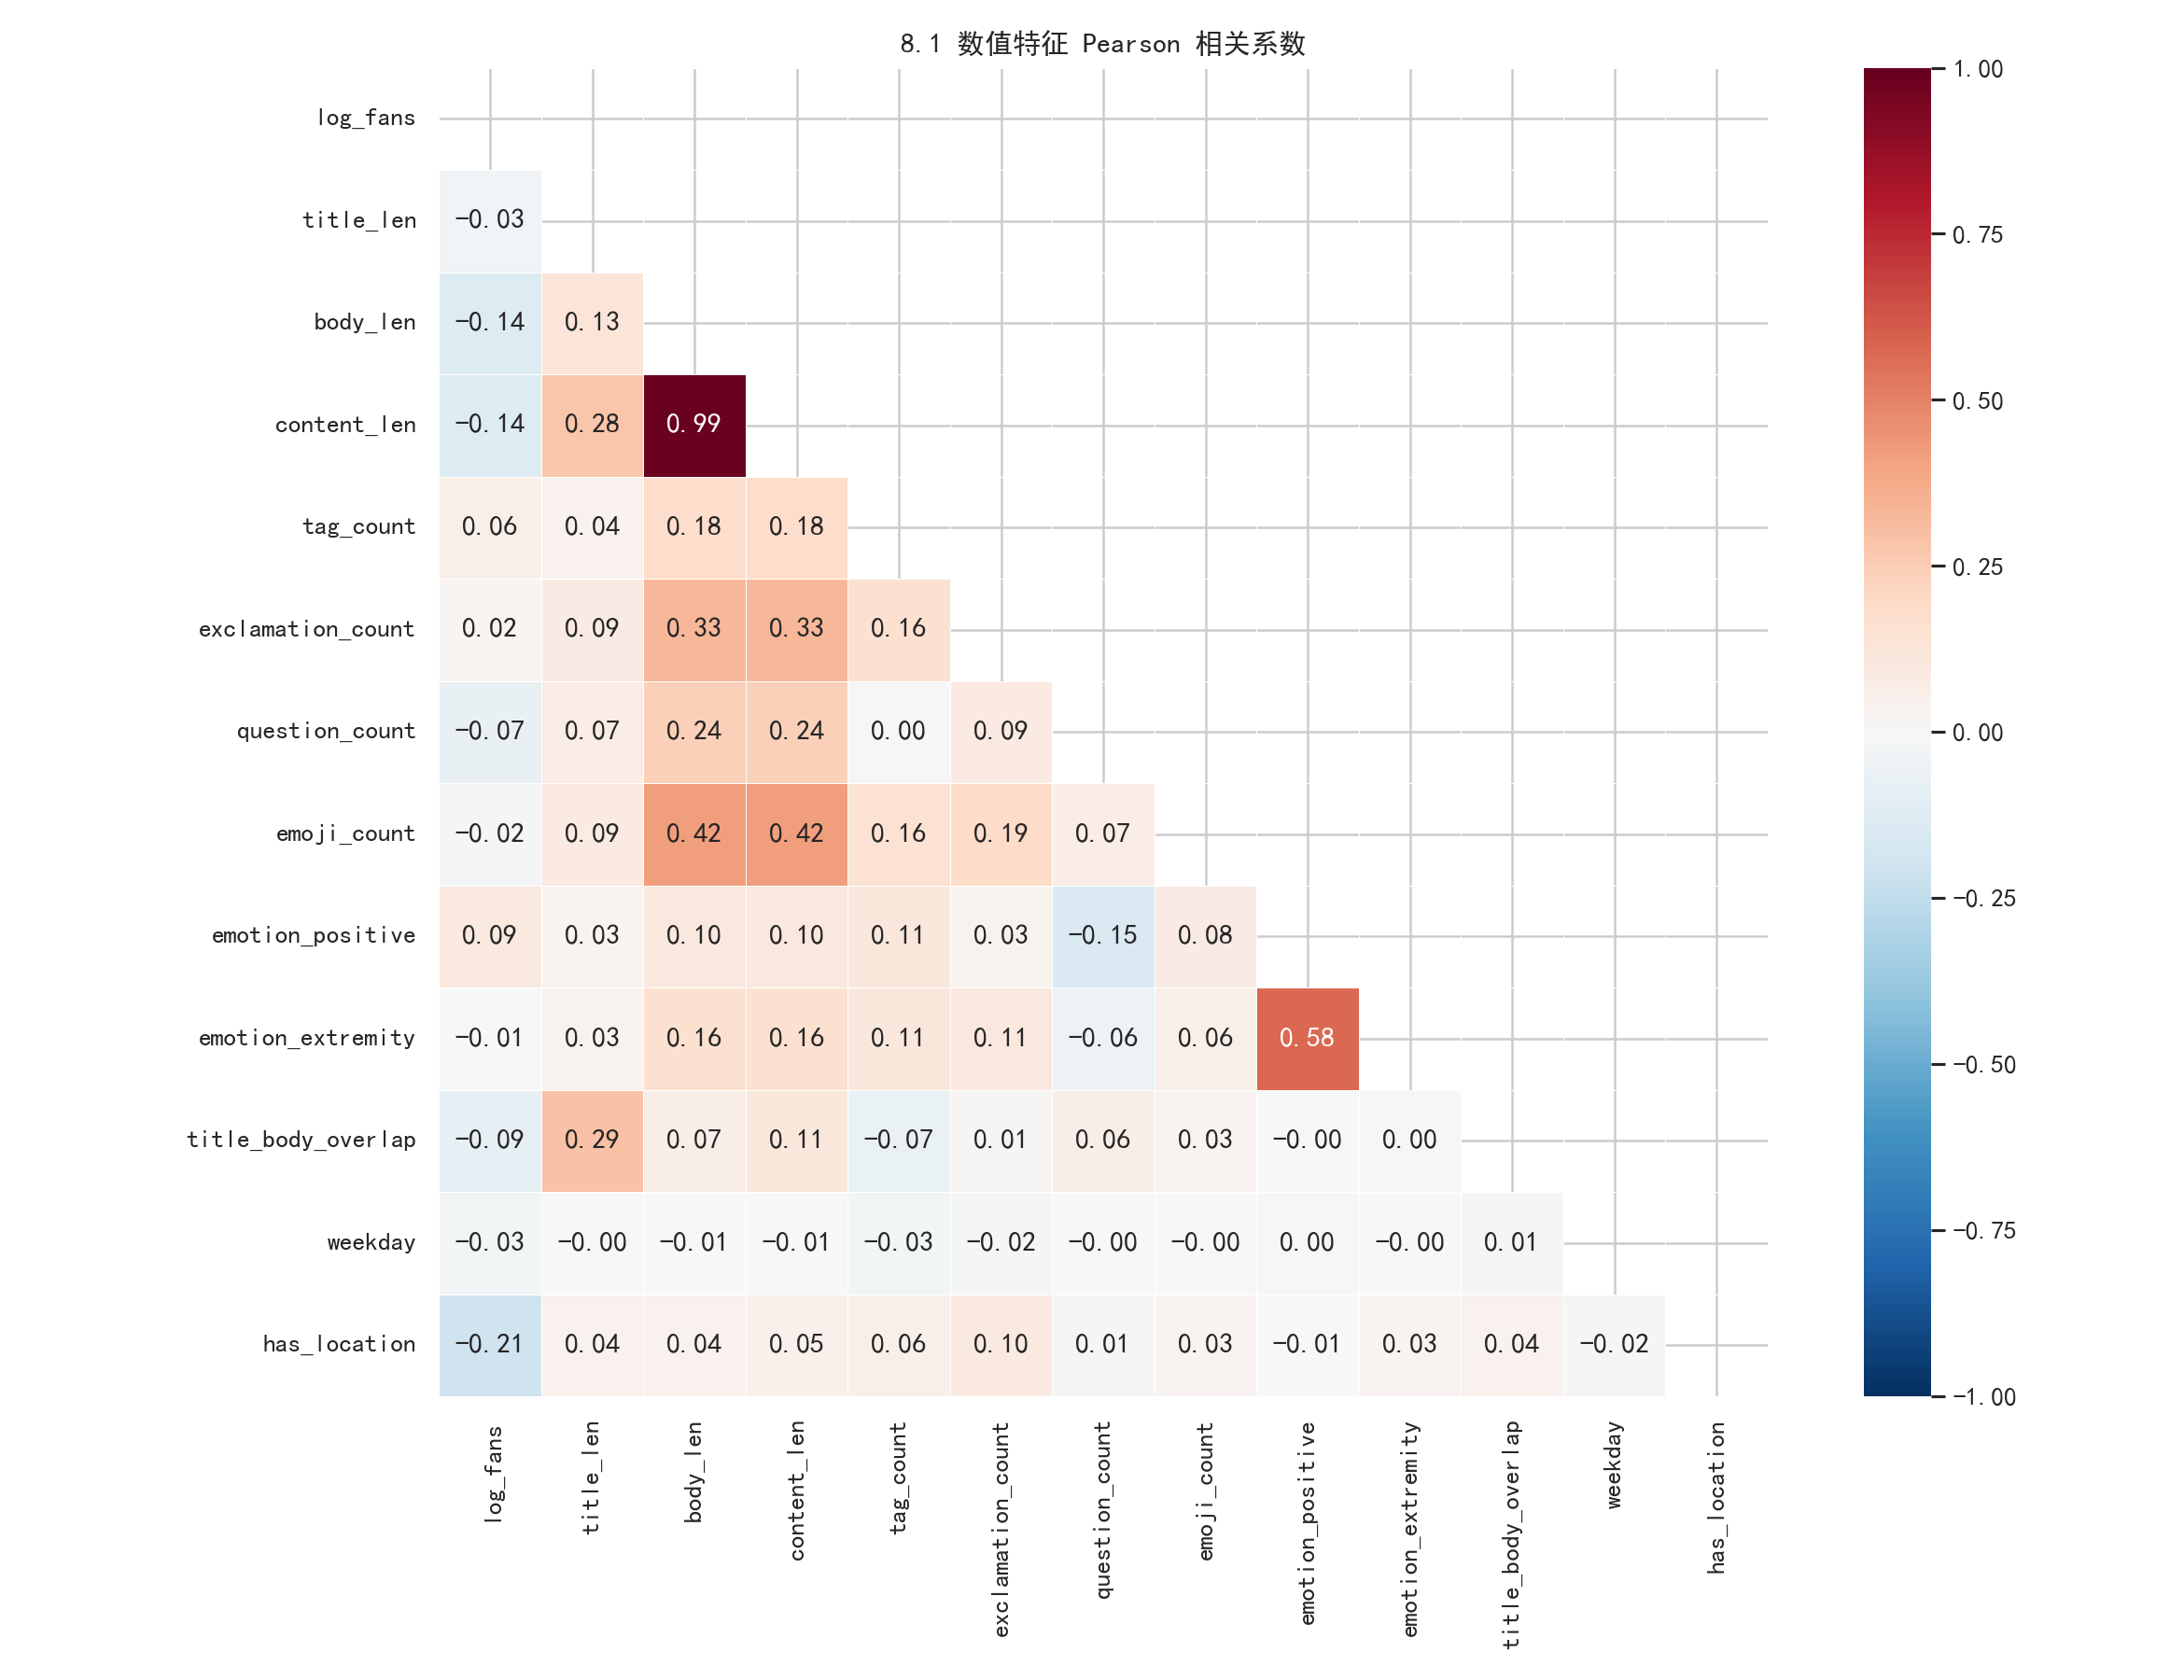
\includegraphics[width=0.92\textwidth]{chapter8_pearson_heatmap.png}
    \caption{数值特征间的Pearson相关系数矩阵}
    \label{fig:chapter8_pearson}
\end{figure}

结果显示，正文长度与全文长度的相关系数达到$r=0.988$，是唯一满足$|r|\geq0.8$的特征对。这一高度相关主要源于全文长度由标题和正文共同构成，属于变量定义带来的机械相关。在后续多变量模型中不宜同时保留正文长度与全文长度，本文建议保留含义更完整的全文长度。其余变量之间未出现绝对相关系数超过0.8的组合，说明除长度变量外，当前特征集合不存在严重的两两线性共线性。需要强调的是，两两相关较低并不能完全排除多变量共线性，后续回归仍应结合VIF进行诊断。

\section{特征与目标变量相关性分析}
本文首先以对数互动量为连续型目标，分别计算各特征的Pearson和Spearman相关系数，并采用Benjamini--Hochberg方法对多重检验的$p$值进行FDR校正。图\ref{fig:chapter8_target}按照Spearman相关系数绝对值展示变量排序。

\begin{figure}[H]
    \centering
    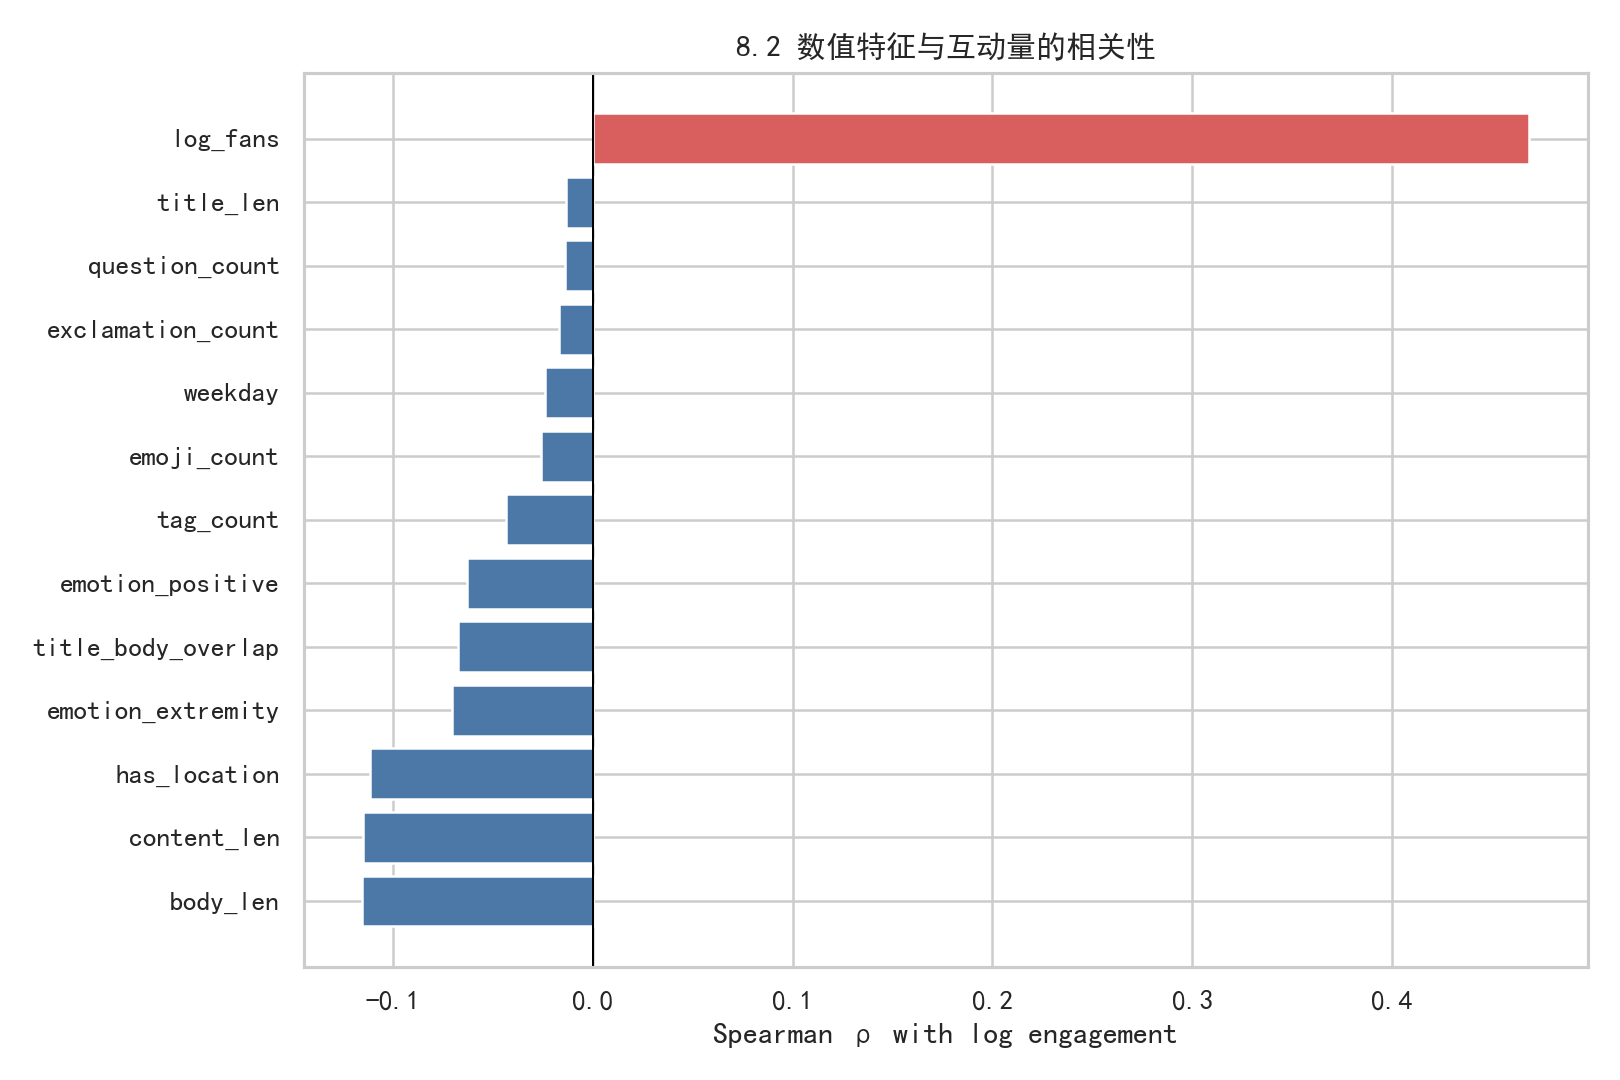
\includegraphics[width=0.82\textwidth]{chapter8_target_ranking.png}
    \caption{数值特征与对数互动量的Spearman相关系数排序}
    \label{fig:chapter8_target}
\end{figure}

粉丝数对数与对数互动量的相关性最强，Pearson相关系数为0.489，Spearman相关系数为0.469，均在FDR校正后显著。这表明发布者既有受众规模仍是笔记互动表现最重要的单一关联因素，但相关系数未达到高度相关水平，笔记热度并不能仅由粉丝基数解释。正文长度和全文长度与互动量呈弱负相关，Spearman系数分别为$-0.116$和$-0.115$；是否具有有效发布地点的系数为$-0.111$。情绪极端程度、标题正文重合度和正向情感概率的Spearman系数分别为$-0.070$、$-0.068$和$-0.063$，方向与第3章的回归结果基本一致，但效应强度较小。标签数量、表情符号、星期、感叹号和问号等变量的绝对相关系数均小于0.05，统计显著性主要受大样本量影响，不宜解释为具有较强的实际作用。

为进一步比较高热度内容，本文将总互动量位于样本前10\%的笔记定义为“爆款”，并对连续特征实施点二列相关、Welch独立样本$t$检验和Mann--Whitney U检验，同时报告Cohen's $d$。粉丝数对数的组间差异最明显：普通组均值为7.613，爆款组均值为9.589，$d=0.696$，属于中等偏大的效应。相比之下，爆款组正文长度和全文长度更短，对应效应量分别为$-0.213$和$-0.211$；标签数量、情绪极端程度与表情数量的效应量绝对值约为0.12至0.14，其余变量的效应量更小。问号数量和星期编码在FDR校正后均未表现出稳定的爆款组差异。

星期编码本身不适合作为严格连续变量解释，因此本文另行进行分组描述。如图\ref{fig:chapter8_weekday}所示，周六和周日的爆款比例分别为10.91\%和10.86\%，周一为10.42\%，周五最低，为8.54\%。该结果说明星期差异主要体现为类别间波动，而非随编码增加或减少的线性趋势。

\begin{figure}[H]
    \centering
    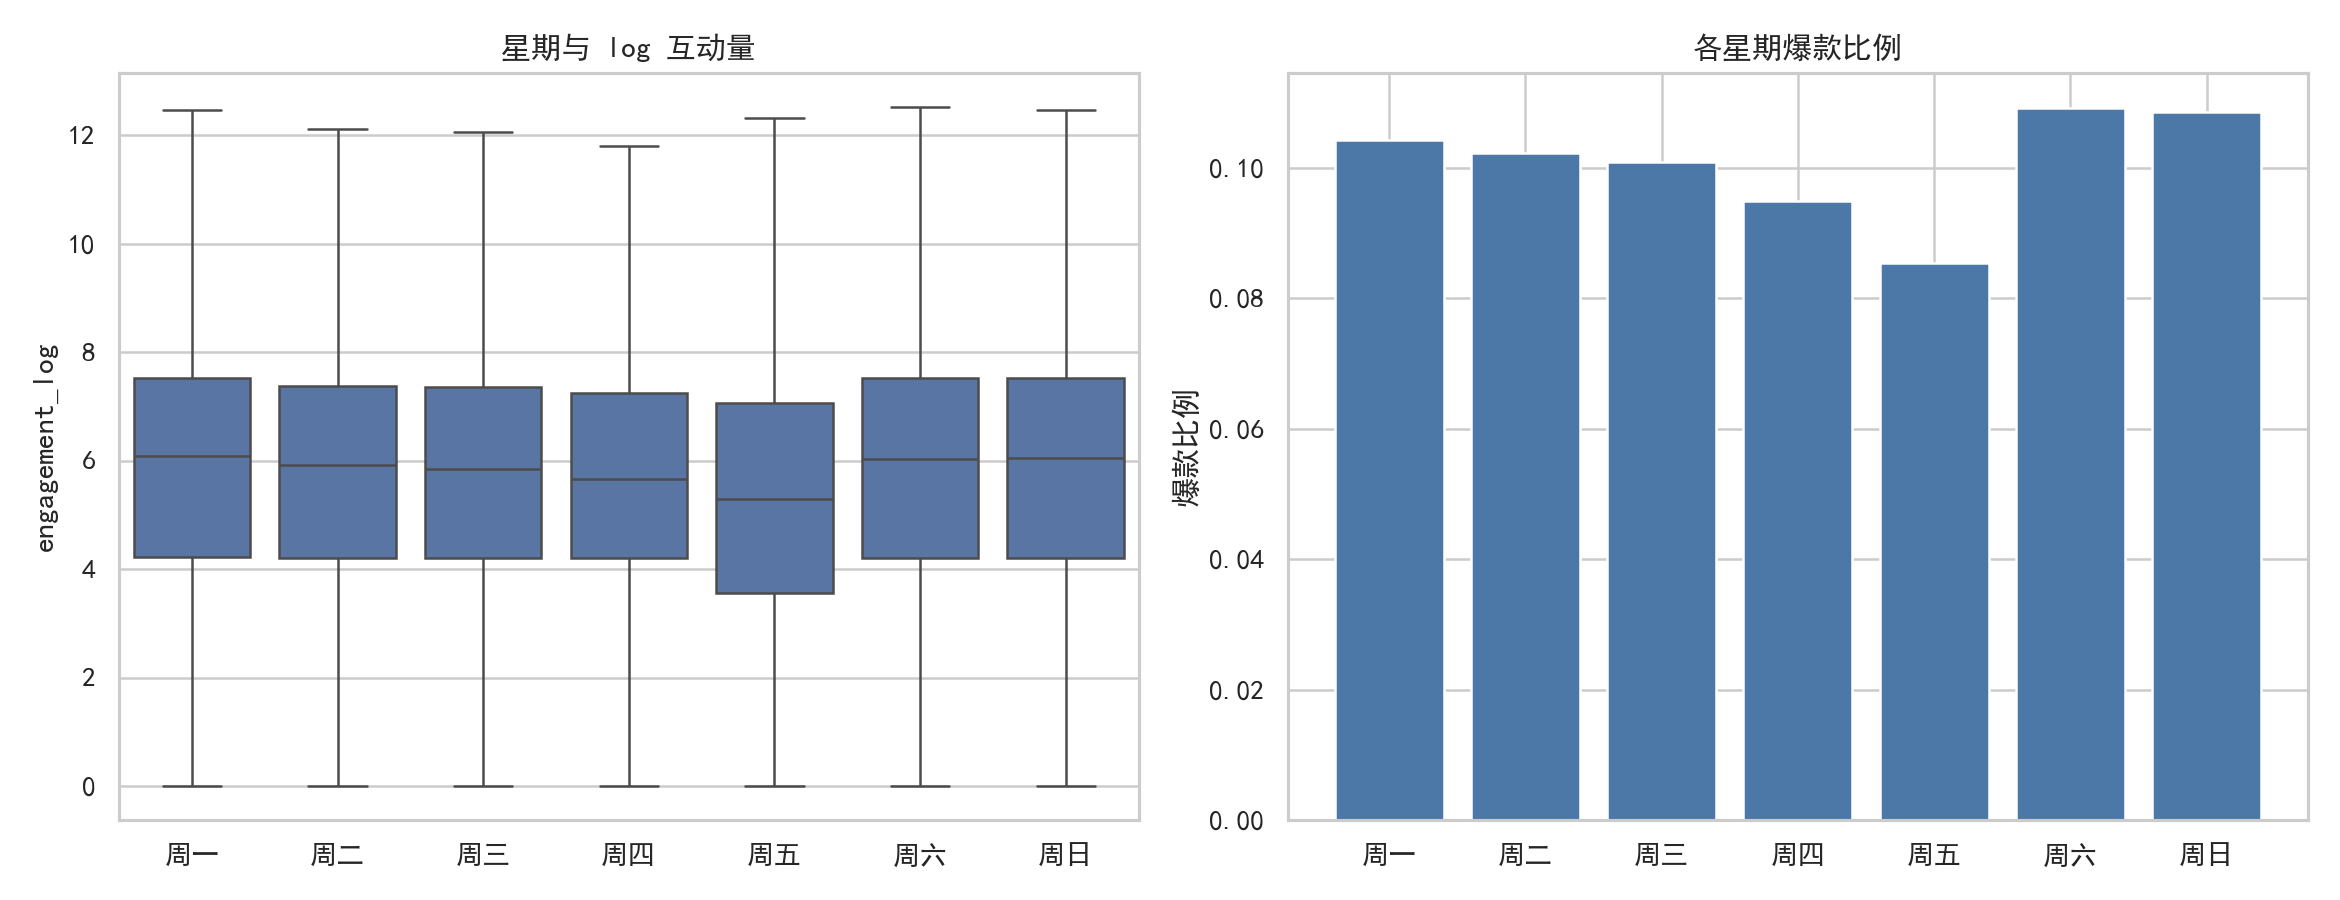
\includegraphics[width=0.9\textwidth]{chapter8_weekday.png}
    \caption{不同星期的互动量分布与爆款比例}
    \label{fig:chapter8_weekday}
\end{figure}

总体而言，粉丝规模是与互动量及爆款状态关联最稳定的特征；文本长度表现出弱负相关；情感、标签及格式变量虽然在大样本下多达到统计显著，但实际效应普遍较弱。因此，后续预测模型不应仅根据$p$值筛选变量，而应综合考虑效应量、非线性结构与变量的理论意义。

\section{非线性关系探索}
线性相关系数可能掩盖阈值、平台期或转折关系。为此，本文对粉丝数对数、全文长度、标签数量、正向情感概率、情绪极端程度和标题正文重合度进行LOWESS局部加权平滑，并将全部有效样本划分为20个分位数组计算组内平均互动。为减少极端值对曲线边界的影响，作图时剔除各自变量上下0.5\%的观测；散点和LOWESS最多随机抽取20,000条记录，而分位数组均值仍使用全部有效数据。

图\ref{fig:chapter8_lowess_main}展示了粉丝规模与文本长度的主要非线性形态。粉丝数对数与互动量总体呈明显正向关系，但曲线并非全程保持相同斜率，说明粉丝增长带来的互动增量存在阶段差异。全文长度曲线则表现出较明显的弯曲：短文本区间互动水平相对较高，随着长度增加先下降，随后在部分较长文本区间趋于平缓或出现局部回升。这与第3.1节在OLS中加入长度平方项后得到的非线性结论相互印证。

\begin{figure}[H]
    \centering
    \begin{minipage}{0.49\textwidth}
        \centering
        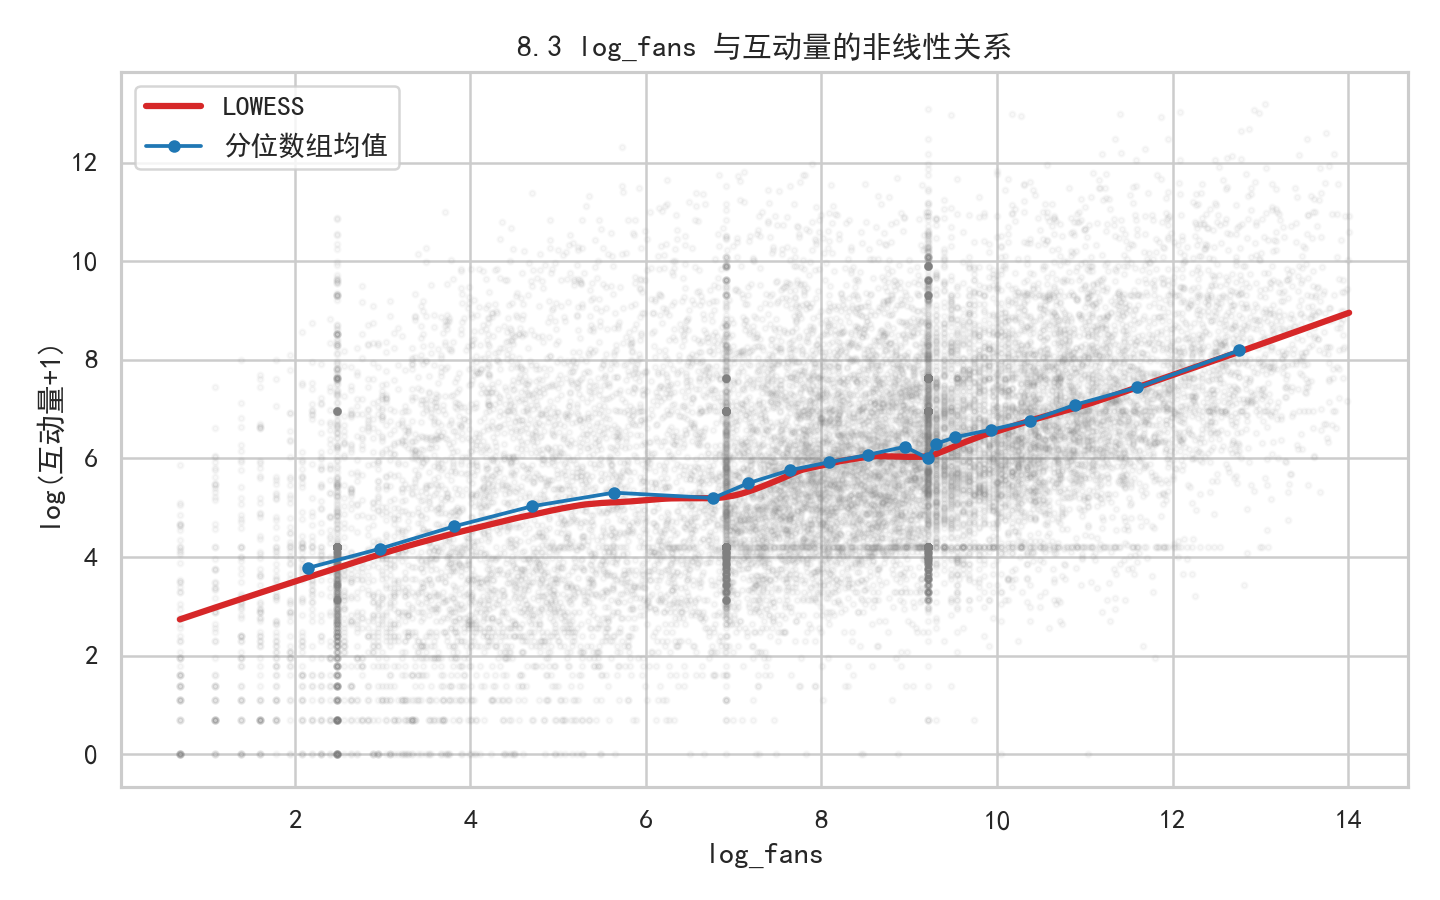
\includegraphics[width=\textwidth]{chapter8_lowess_fans.png}
    \end{minipage}
    \begin{minipage}{0.49\textwidth}
        \centering
        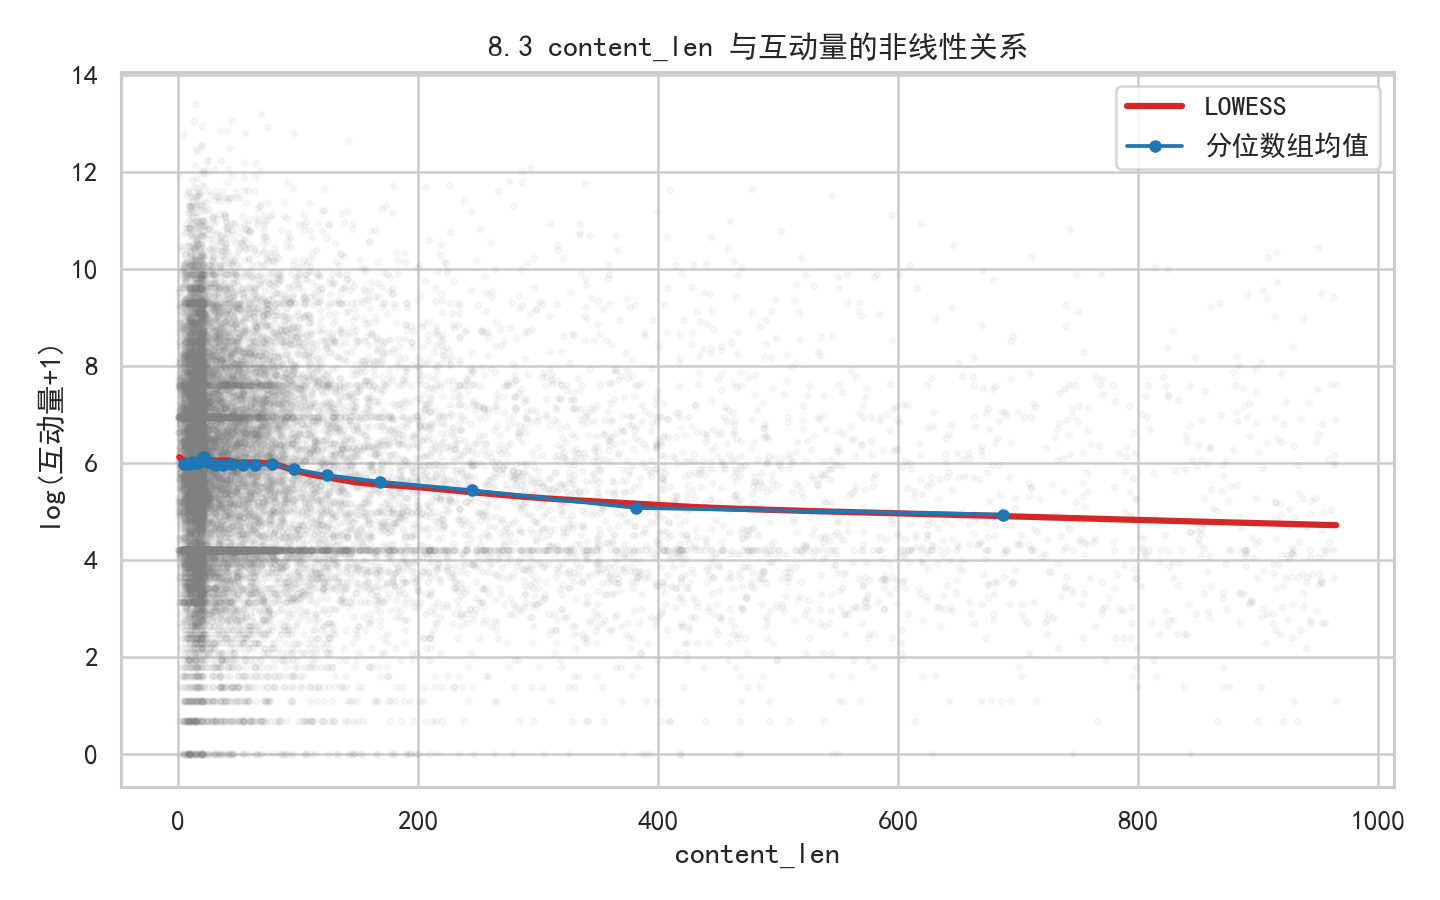
\includegraphics[width=\textwidth]{chapter8_lowess_content.png}
    \end{minipage}
    \caption{粉丝规模与全文长度的LOWESS非线性关系}
    \label{fig:chapter8_lowess_main}
\end{figure}

情绪极端程度的LOWESS结果见图\ref{fig:chapter8_lowess_emotion}。总体趋势显示，越偏离中性区间，平均对数互动量越低，但局部区间存在波动。这说明情感效应不宜简单表述为严格线性下降，更适合在后续模型中使用二次项、限制性立方样条或树模型检验。标签数量、正向情感概率和标题正文重合度也呈现不同程度的局部弯曲，但其总体变化幅度明显小于粉丝规模和文本长度。

\begin{figure}[H]
    \centering
    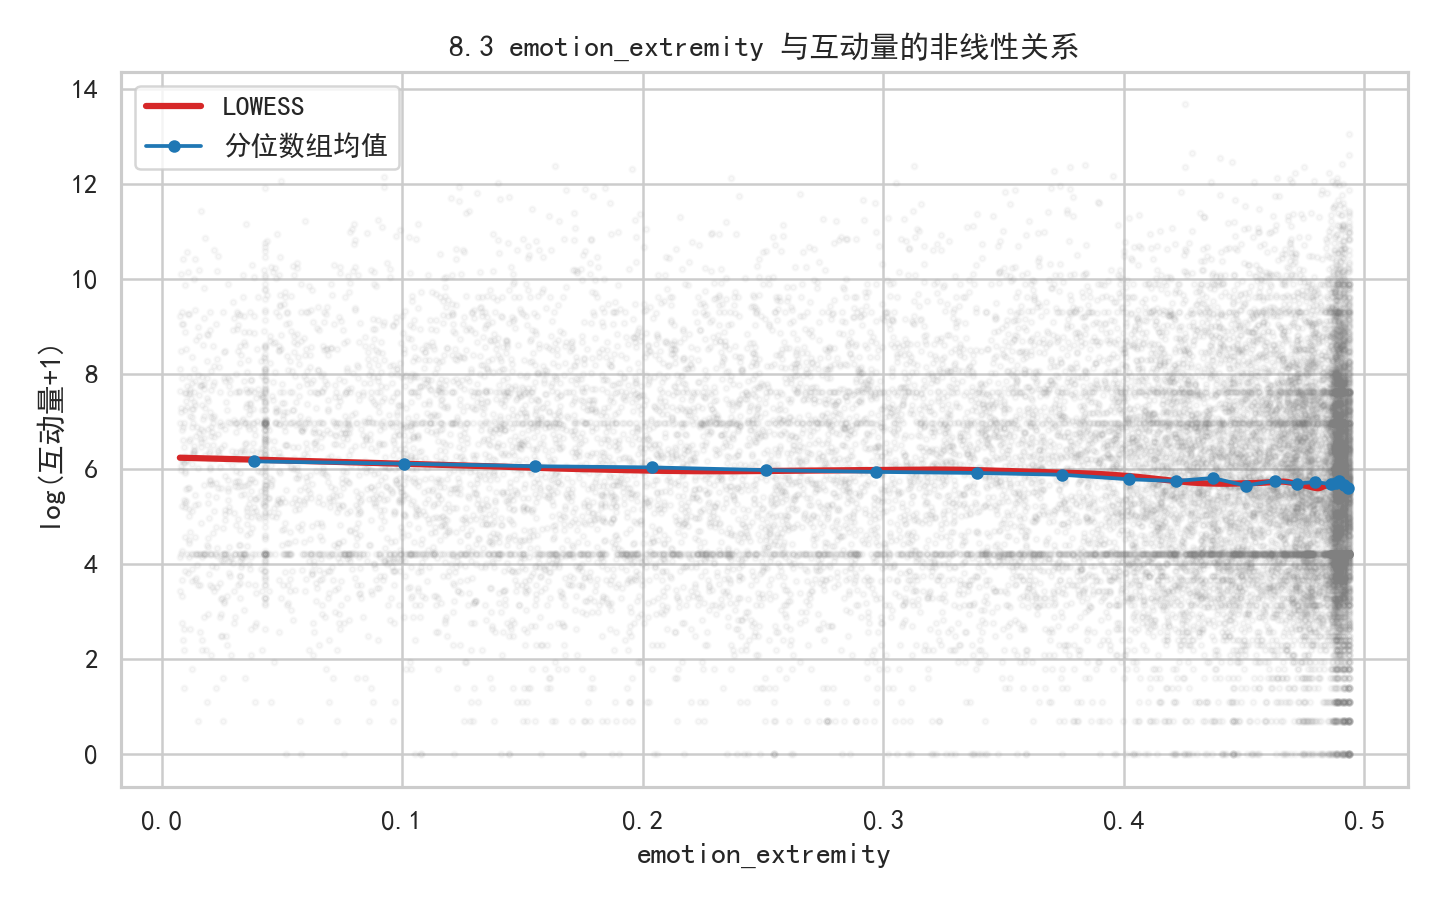
\includegraphics[width=0.78\textwidth]{chapter8_lowess_emotion.png}
    \caption{情绪极端程度与互动量的LOWESS关系}
    \label{fig:chapter8_lowess_emotion}
\end{figure}

需要指出，LOWESS属于探索性可视化方法，曲线形态不能直接证明因果关系。账号粉丝基础、内容类别、采集时间以及平台推荐机制都可能同时影响文本特征和互动结果。因此，本节的非线性发现主要用于为后续模型设定提供依据，而不将曲线转折点直接解释为普遍适用的内容运营最优值。

\chapterimage{chapter_head_2.pdf}
\chapter{特征选择与重要性评估}

\section{筛选原则与实际输入特征}
第8章同时报告相关系数、FDR校正后的显著性、组间检验和效应量。由于样本量较大，较小的差异也可能产生很低的$p$值，因此本研究没有采用“$p<0.05$即保留、否则删除”的单一规则。筛选时优先考虑变量是否能在发布前获得、是否存在目标泄漏、缺失程度、效应量与业务含义，并以非线性模型检验弱单变量特征的组合价值。

正文长度与全文长度的Pearson相关系数达到0.988，属于变量定义造成的机械共线，因此统一模型不同时纳入两者。后续分类与回归实验最终使用相同的10项输入：粉丝量对数、标题长度、正文长度、标签数、感叹号数、问号数、Emoji数、情感得分、星期和是否标注发布地。点赞、收藏和评论共同构成目标变量，不作为输入；图片、认证、用户历史与热点变量则因当前数据不足而不进入模型。

\section{已实施的模型重要性评估}
分类实验报告随机森林的基于不纯度的重要性：粉丝量对数为0.310，情感得分、正文长度和标题长度依次为0.181、0.131和0.108，四项合计约占73\%。回归实验对最佳梯度提升树使用测试集排列重要性；打乱粉丝量对数使对数尺度误差增加2.620，星期、正文长度、情感得分和是否标注发布地的重要性均值分别为0.154、0.136、0.136和0.105。两类任务均将粉丝基础识别为主要预测信号，并显示内容与上下文特征提供一定增量。

两种重要性的定义与量纲不同，不能直接相加或据此生成未经验证的“综合得分”；不纯度重要性还可能偏向可分裂点较多的变量，排列重要性也会在相关特征间分摊贡献。本轮没有实施SHAP、Lasso筛选或将多种重要性归一化后加权，因此不报告相应结果。以上数值用于解释模型的预测依据，不表示改变某一特征会造成同等幅度的热度变化。
